\hypertarget{sec-interpretation}{%
\chapter{Model Interpretation}\label{sec-interpretation}}

\vspace{-15mm}\addtocontents{toc}{\textit{Susanne Dandl, Przemysław Biecek, Giuseppe Casalicchio and Marvin N. Wright}}

\textbf{Susanne Dandl} \newline  \emph{Ludwig-Maximilians-Universität
München, and Munich Center for Machine Learning (MCML)}

\textbf{Przemysław Biecek} \newline  \emph{MI2.AI, Warsaw University of
Technology, and University of Warsaw}

\textbf{Giuseppe Casalicchio} \newline 
\emph{Ludwig-Maximilians-Universität München, and Munich Center for
Machine Learning (MCML), and Essential Data Science Training GmbH}

\textbf{Marvin N. Wright} \newline  \emph{Leibniz Institute for
Prevention Research and Epidemiology -- BIPS, and University of Bremen,
and University of Copenhagen} \newline \newline 

The increasing availability of data and software frameworks to create
predictive models has allowed the widespread adoption of ML in many
applications. However, high predictive performance of such models often
comes at the cost of interpretability\index{interpretability}. Many
models are called a `black box\index{black box}' as the decision-making
process behind their predictions is often not immediately interpretable.
This lack of explanation can decrease trust in ML and may create
barriers to the adoption of predictive models, especially in critical
applications such as medicine, engineering, and finance (Lipton 2018).

In recent years, many interpretation methods have been developed that
allow developers to `peek' inside these models and produce explanations
to, for example, understand how features are used by the model to make
predictions (Guidotti et al. 2018). Interpretation methods can be
valuable from multiple perspectives:

\begin{enumerate}
\def\labelenumi{\arabic{enumi}.}
\tightlist
\item
  To gain global insights into a model, for example, to identify which
  features were the most important overall or how the features act on
  the predictions.
\item
  To improve the model if flaws are identified (in the data or model),
  for example, if the model depends on one feature unexpectedly.
\item
  To understand and control individual predictions, for example, to
  identify how a given prediction may change if a feature is altered.
\item
  To assess algorithmic fairness\index{algorithmic fairness}, for
  example, to inspect whether the model adversely affects certain
  subpopulations or individuals (see Chapter~\ref{sec-fairness}).
\end{enumerate}

In this chapter, we will look at model-agnostic (i.e., can be applied to
any model) interpretable machine
learning\index{interpretable machine learning}{\marginnote{\begin{footnotesize}Interpretable
Machine Learning\end{footnotesize}}} (IML) methods that can be used to
understand models post hoc\index{post hoc} (after they have been
trained). We will focus on methods implemented in three R packages that
nicely interface with \texttt{mlr3}:
\href{https://cran.r-project.org/package=iml}{\texttt{iml}}
(Section~\ref{sec-iml}),
\href{https://cran.r-project.org/package=counterfactuals}{\texttt{counterfactuals}}
(Section~\ref{sec-counterfactuals}), and
\href{https://cran.r-project.org/package=DALEX}{\texttt{DALEX}}
(Section~\ref{sec-dalex}).

\texttt{iml} and \texttt{DALEX} offer similar functionality but differ
in design choices in that \texttt{iml} makes use of the \texttt{R6}
class system whereas \texttt{DALEX} is based on the S3 class system.
\texttt{counterfactuals} also uses the \texttt{R6} class system. In
contrast to \texttt{iml} and \texttt{counterfactuals}, \texttt{DALEX}
focuses on comparing multiple predictive models, usually of different
types. We will only provide a brief overview of the methodology
discussed below, we recommend Molnar (2022) as a comprehensive
introductory book about IML.

As a running example throughout this chapter, we will consider a
gradient boosting machine (GBM) fit on half the features in the
\texttt{"german\_credit"} task. In practice, we would tune the
hyperparameters of GBM as discussed in Chapter~\ref{sec-optimization}
and perform feature selection as discussed in
Chapter~\ref{sec-feature-selection} to select the most relevant
features. However, for the sake of simplicity, we utilize an untuned GBM
in these examples as it exhibited satisfactory performance even without
fine-tuning.

\begin{Shaded}
\begin{Highlighting}[]
\FunctionTok{library}\NormalTok{(mlr3verse)}
\NormalTok{tsk\_german }\OtherTok{=} \FunctionTok{tsk}\NormalTok{(}\StringTok{"german\_credit"}\NormalTok{)}\SpecialCharTok{$}\FunctionTok{select}\NormalTok{(}
  \AttributeTok{cols =} \FunctionTok{c}\NormalTok{(}\StringTok{"duration"}\NormalTok{, }\StringTok{"amount"}\NormalTok{, }\StringTok{"age"}\NormalTok{, }\StringTok{"status"}\NormalTok{, }\StringTok{"savings"}\NormalTok{, }\StringTok{"purpose"}\NormalTok{,}
  \StringTok{"credit\_history"}\NormalTok{, }\StringTok{"property"}\NormalTok{, }\StringTok{"employment\_duration"}\NormalTok{, }\StringTok{"other\_debtors"}\NormalTok{))}
\NormalTok{split }\OtherTok{=} \FunctionTok{partition}\NormalTok{(tsk\_german)}
\NormalTok{lrn\_gbm }\OtherTok{=} \FunctionTok{lrn}\NormalTok{(}\StringTok{"classif.gbm"}\NormalTok{, }\AttributeTok{predict\_type =} \StringTok{"prob"}\NormalTok{)}
\NormalTok{lrn\_gbm}\SpecialCharTok{$}\FunctionTok{train}\NormalTok{(tsk\_german, }\AttributeTok{row\_ids =}\NormalTok{ split}\SpecialCharTok{$}\NormalTok{train)}
\end{Highlighting}
\end{Shaded}

\begin{tcolorbox}[enhanced jigsaw, opacitybacktitle=0.6, rightrule=.15mm, opacityback=0, arc=.35mm, breakable, titlerule=0mm, colframe=quarto-callout-tip-color-frame, coltitle=black, bottomrule=.15mm, toprule=.15mm, colback=white, colbacktitle=quarto-callout-tip-color!10!white, bottomtitle=1mm, toptitle=1mm, title=\textcolor{quarto-callout-tip-color}{\faLightbulb}\hspace{0.5em}{Performance-based Interpretation Methods Require Test Data}, leftrule=.75mm, left=2mm]

Performance-based interpretation methods such as permutation feature
importance (Section~\ref{sec-feat-importance}) rely on measuring the
generalization performance. Hence, they should be computed on an
independent test set to decrease bias in estimation (see
Chapter~\ref{sec-performance}).

However, the differences in interpretation between training and test
data are less pronounced (Molnar et al. 2022) in prediction-based
methods that do not require performance estimation such as ICE/PD
(Section~\ref{sec-feature-effects}) or Shapley values
(Section~\ref{sec-shapley}).

\end{tcolorbox}

\hypertarget{sec-iml}{%
\section{The iml Package}\label{sec-iml}}

\index{\texttt{iml}}\href{https://cran.r-project.org/package=iml}{\texttt{iml}}
(Molnar, Bischl, and Casalicchio 2018) implements a unified interface
for a variety of model-agnostic interpretation methods that facilitate
the analysis and interpretation of machine learning models. \texttt{iml}
supports machine learning models (for classification or regression)
fitted by \emph{any} R package, and in particular all \texttt{mlr3}
models are supported by wrapping learners in an
\href{https://www.rdocumentation.org/packages/iml/topics/Predictor}{\texttt{Predictor}}
object, which unifies the input-output behavior of the trained models.
This object contains the prediction model as well as the data used for
analyzing the model and producing the desired explanation. We construct
the \texttt{Predictor} object using our trained learner and heldout test
data:

\begin{Shaded}
\begin{Highlighting}[]
\FunctionTok{library}\NormalTok{(iml)}

\CommentTok{\# features in test data}
\NormalTok{credit\_x }\OtherTok{=}\NormalTok{ tsk\_german}\SpecialCharTok{$}\FunctionTok{data}\NormalTok{(}\AttributeTok{rows =}\NormalTok{ split}\SpecialCharTok{$}\NormalTok{test,}
  \AttributeTok{cols =}\NormalTok{ tsk\_german}\SpecialCharTok{$}\NormalTok{feature\_names)}
\CommentTok{\# target in test data}
\NormalTok{credit\_y }\OtherTok{=}\NormalTok{ tsk\_german}\SpecialCharTok{$}\FunctionTok{data}\NormalTok{(}\AttributeTok{rows =}\NormalTok{ split}\SpecialCharTok{$}\NormalTok{test,}
  \AttributeTok{cols =}\NormalTok{ tsk\_german}\SpecialCharTok{$}\NormalTok{target\_names)}

\NormalTok{predictor }\OtherTok{=}\NormalTok{ Predictor}\SpecialCharTok{$}\FunctionTok{new}\NormalTok{(lrn\_gbm, }\AttributeTok{data =}\NormalTok{ credit\_x, }\AttributeTok{y =}\NormalTok{ credit\_y)}
\end{Highlighting}
\end{Shaded}

With our \texttt{Predictor} setup we can now consider different model
interpretation methods.

\hypertarget{sec-feat-importance}{%
\subsection{\texorpdfstring{Feature
Importance\index{feature importance}}{Feature Importance}}\label{sec-feat-importance}}

When deploying a model in practice, it is often of interest to know
which features contribute the most to the \emph{predictive performance}
of the model. This can be useful to better understand the problem at
hand and the relationship between features and target. In model
development, this can be used to filter features
(Section~\ref{sec-fs-filter}) that do not contribute a lot to the
model's predictive ability. In this book, we use the term `feature
importance' to describe global methods that calculate a single score per
feature that reflect the importance regarding a given quantity of
interest, e.g., model performance, thus allowing features to be ranked.

One of the most popular feature importance methods is the permutation
feature
importance\index{permutation feature importance}{\marginnote{\begin{footnotesize}Permutation
Feature Importance\end{footnotesize}}} (PFI), originally introduced by
Breiman (2001a) for random forests\index{random forest} and adapted by
Fisher, Rudin, and Dominici (2019) as a model-agnostic feature
importance measure (originally termed, `model reliance'). Feature
permutation is the process of randomly shuffling observed values for a
single feature in a dataset. This removes the original dependency
structure of the feature with the target variable and with all other
features while maintaining the marginal distribution of the feature. The
PFI measures the change in the model performance before (original model
performance) and after (permuted model performance) permuting a feature.
If a feature is not important, then there will be little change in model
performance after permuting that feature. Conversely, we would expect a
clear decrease in model performance if the feature is more important. It
is generally recommended to repeat the permutation process and aggregate
performance changes over multiple repetitions to decrease randomness in
results.

PFI is run in \texttt{iml} by constructing an object of class
\href{https://www.rdocumentation.org/packages/iml/topics/FeatureImp}{\texttt{FeatureImp}}
and specifying the performance measure, below we use classification
error. By default, the permutation is repeated five times to keep
computation time low (this can be changed with \texttt{n.repetitions}
when calling the constructor \texttt{\$new()}, below we set
\texttt{n.repetitions\ =\ 100}) and in each repetition, the importance
value corresponding to the change in the classification error is
calculated. The \texttt{\$plot()} method shows the median of the five
resulting importance values (as a point) and the boundaries of the error
bars in the plot refer to the 5\% and 95\% quantiles of the importance
values (Figure~\ref{fig-iml-pfi}).

\begin{tcolorbox}[enhanced jigsaw, opacitybacktitle=0.6, rightrule=.15mm, opacityback=0, arc=.35mm, breakable, titlerule=0mm, colframe=quarto-callout-tip-color-frame, coltitle=black, bottomrule=.15mm, toprule=.15mm, colback=white, colbacktitle=quarto-callout-tip-color!10!white, bottomtitle=1mm, toptitle=1mm, title=\textcolor{quarto-callout-tip-color}{\faLightbulb}\hspace{0.5em}{Increase the Number of Repetitions to Obtain Useful Error Bars}, leftrule=.75mm, left=2mm]

The default number of repetitions when constructing a
\texttt{FeatureImp} object is \texttt{5}. However, the number of
repetitions should be increased if you want to obtain useful error bars
from the resulting plot.

\end{tcolorbox}

\begin{Shaded}
\begin{Highlighting}[]
\NormalTok{importance }\OtherTok{=}\NormalTok{ FeatureImp}\SpecialCharTok{$}\FunctionTok{new}\NormalTok{(predictor, }\AttributeTok{loss =} \StringTok{"ce"}\NormalTok{, }\AttributeTok{n.repetitions =} \DecValTok{100}\NormalTok{)}
\NormalTok{importance}\SpecialCharTok{$}\FunctionTok{plot}\NormalTok{()}
\end{Highlighting}
\end{Shaded}

\begin{figure}

{\centering 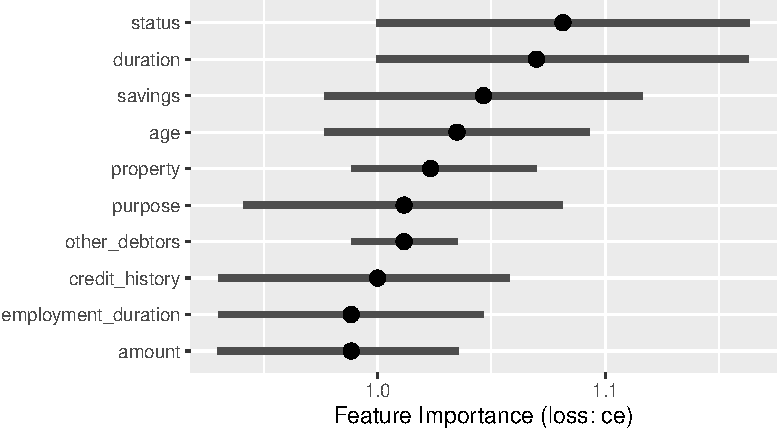
\includegraphics[width=1\textwidth,height=\textheight]{chapters/chapter12/model_interpretation_files/figure-pdf/fig-iml-pfi-1.pdf}

}

\caption{\label{fig-iml-pfi}Permutation feature importance (PFI). Points
indicate the median and bars the 5\% and 95\% quantiles of the PFI over
five repetitions of the permutation process.}

\end{figure}

The plot automatically ranks features from most (largest median
performance change) to least (smallest median performance change)
important. In Figure~\ref{fig-iml-pfi}, the feature \texttt{status} is
most important, if we permute the \texttt{status} column in the data the
classification error of our model increases by a factor of around 1.08.
By default, \texttt{FeatureImp} calculates the \emph{ratio} of the model
performance before and after permutation as an importance value; the
\emph{difference} of the performance measures can be returned by passing
\texttt{compare\ =\ "difference"} when calling \texttt{\$new()}.

\hypertarget{sec-feature-effects}{%
\subsection{Feature Effects}\label{sec-feature-effects}}

Feature effect\index{feature effect} methods describe how or to what
extent a feature contributes towards the \emph{model predictions} by
analyzing how the predictions change when changing a feature. These
methods can be distinguished between local and global feature effect
methods. Global feature effect methods refer to how a prediction changes
\emph{on average} when a feature is changed. In contrast, local feature
effect methods address the question of how a \emph{single} prediction of
a given observation changes when a feature value is changed. To a
certain extent, local feature effect methods can reveal interactions in
the model that become visible when the local effects are heterogeneous,
i.e., if changes in the local effect are different across the
observations.

Partial
dependence\index{partial dependence}{\marginnote{\begin{footnotesize}Partial
Dependence\end{footnotesize}}} (PD) plots (Friedman 2001) can be used to
visualize global feature effects by visualizing how model predictions
change on average when varying the values of a given feature of
interest.

Individual conditional
expectation\index{individual conditional expectation}{\marginnote{\begin{footnotesize}Individual
Conditional Expectation\end{footnotesize}}} (ICE) curves (Goldstein et
al. 2015) (a.k.a. Ceteris Paribus
Effects\index{ceteris paribus|see{individual conditional expectation (ICE) curves}})
are a local feature effects method that display how the prediction of a
\emph{single} observation changes when varying a feature of interest,
while all other features stay constant. Goldstein et al. (2015)
demonstrated that the PD plot is the average of ICE curves. ICE curves
are constructed by taking a single observation and feature of interest,
and then replacing the feature's value with another value and plotting
the new prediction, this is then repeated for many feature values (e.g.,
across an equidistant grid of the feature's value range). The x-axis of
an ICE curve visualizes the set of replacement feature values and the
y-axis is the model prediction. Each ICE curve is a local explanation
that assesses the feature effect of a single observation on the model
prediction. An ICE plot contains one ICE curve (line) per observation.
If the ICE curves are heterogeneous, i.e., not parallel, then the model
may have estimated an interaction involving the considered feature.

\begin{tcolorbox}[enhanced jigsaw, opacitybacktitle=0.6, rightrule=.15mm, opacityback=0, arc=.35mm, breakable, titlerule=0mm, colframe=quarto-callout-tip-color-frame, coltitle=black, bottomrule=.15mm, toprule=.15mm, colback=white, colbacktitle=quarto-callout-tip-color!10!white, bottomtitle=1mm, toptitle=1mm, title=\textcolor{quarto-callout-tip-color}{\faLightbulb}\hspace{0.5em}{Feature Effects Can Be Non-Linear}, leftrule=.75mm, left=2mm]

Feature effects are very similar to regression coefficients, \(\beta\),
in linear models which offer interpretations such as ``if you increase
this feature by one unit, your prediction increases on average by
\(\beta\) if all other features stay constant''. However, feature
effects are not limited to linear effects and can be applied to any type
of predictive model.

\end{tcolorbox}

Let us put this into practice by considering how the feature
\texttt{amount} influences the predictions in our subsetted credit
classification task. Below we initialize an object of class
\href{https://www.rdocumentation.org/packages/iml/topics/FeatureEffect}{\texttt{FeatureEffect}}
by passing the feature name of interest and the feature effect method,
we use \texttt{"pdp+ice"} to indicate that we want to visualize ICE
curves with a PD plot (average of the ICE curves). We recommend always
plotting PD and ICE curves together as PD plots on their own could mask
heterogeneous effects. We use \texttt{\$plot()} to visualize the results
(Figure~\ref{fig-iml-pdice}).

\begin{Shaded}
\begin{Highlighting}[]
\NormalTok{effect }\OtherTok{=}\NormalTok{ FeatureEffect}\SpecialCharTok{$}\FunctionTok{new}\NormalTok{(predictor, }\AttributeTok{feature =} \StringTok{"amount"}\NormalTok{,}
  \AttributeTok{method =} \StringTok{"pdp+ice"}\NormalTok{)}
\NormalTok{effect}\SpecialCharTok{$}\FunctionTok{plot}\NormalTok{()}
\end{Highlighting}
\end{Shaded}

\begin{figure}[H]

{\centering 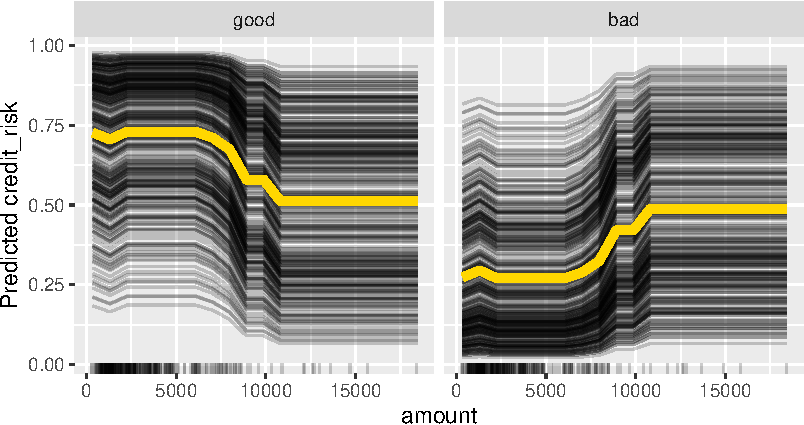
\includegraphics[width=1\textwidth,height=\textheight]{chapters/chapter12/model_interpretation_files/figure-pdf/fig-iml-pdice-1.pdf}

}

\caption{\label{fig-iml-pdice}Partial dependence (PD) plot (yellow) and
individual conditional expectation (ICE) curves (black) that show how
the credit amount affects the predicted credit risk.}

\end{figure}

Figure~\ref{fig-iml-pdice} shows that if the \texttt{amount} is smaller
than roughly 10,000 then on average there is a high chance that the
predicted creditworthiness will be \texttt{good}. Furthermore, the ICE
curves are roughly parallel, meaning that there do not seem to be strong
interactions present where \texttt{amount} is involved.

\hypertarget{surrogate-models-1}{%
\subsection{Surrogate Models}\label{surrogate-models-1}}

Interpretable models such as decision trees or linear models can be used
as surrogate models\index{surrogate model} to approximate or mimic an,
often very complex, black box model. Inspecting the surrogate model can
provide insights into the behavior of a black box model, for example by
looking at the model coefficients in a linear regression or splits in a
decision tree. We differentiate between local surrogate models, which
approximate a model locally around a specific data point of interest,
and global surrogate models which approximate the model across the
entire input space (Ribeiro, Singh, and Guestrin 2016; Molnar 2022).

The features used to train a surrogate model are usually the same
features used to train the black box model or at least data with the
same distribution to ensure a representative input space. However, the
target used to train the surrogate model is the predictions obtained
from the black box model, not the real outcome of the underlying data.
Hence, conclusions drawn from the surrogate model are only valid if the
surrogate model approximates the black box model very well (i.e., if the
model fidelity is high). It is therefore also important to measure and
report the approximation error of the surrogate model.

The data used to train the black box model may be very complex or
limited, making it challenging to directly train a well-performing
interpretable model on that data. Instead, we can use the black box
model to generate new labeled data in specific regions of the input
space with which we can augment the original data. The augmented data
can then be used to train an interpretable model that captures and
explains the relationships learned by the black box model (in specific
regions) or to identify flaws or unexpected behavior.

\hypertarget{global-surrogate-model}{%
\subsubsection{Global Surrogate Model}\label{global-surrogate-model}}

\index{surrogate model!global}Initializing the
\href{https://www.rdocumentation.org/packages/iml/topics/TreeSurrogate}{\texttt{TreeSurrogate}}
class fits a conditional inference tree
(\href{https://www.rdocumentation.org/packages/partykit/topics/ctree}{\texttt{ctree()}})
surrogate model to the predictions from our trained model. This class
extracts the decision rules created by the tree surrogate and the
\texttt{\$plot()} method visualizes the distribution of the predicted
outcomes from each terminal node. Below, we pass \texttt{maxdepth\ =\ 2}
to the constructor to build a tree with two binary splits, yielding four
terminal nodes.

\begin{Shaded}
\begin{Highlighting}[]
\NormalTok{tree\_surrogate }\OtherTok{=}\NormalTok{ TreeSurrogate}\SpecialCharTok{$}\FunctionTok{new}\NormalTok{(predictor, }\AttributeTok{maxdepth =}\NormalTok{ 2L)}
\end{Highlighting}
\end{Shaded}

Before inspecting this model, we need to first check if the surrogate
model approximates the prediction model accurately, which we can assess
by comparing the predictions of the tree surrogate and the predictions
of the black box model. For example, we could quantify the number of
matching predictions and measure the accuracy of the surrogate in
predicting the predictions of the black box GBM model:

\begin{Shaded}
\begin{Highlighting}[]
\NormalTok{pred\_surrogate }\OtherTok{=}\NormalTok{ tree\_surrogate}\SpecialCharTok{$}\FunctionTok{predict}\NormalTok{(credit\_x, }\AttributeTok{type =} \StringTok{"class"}\NormalTok{)}\SpecialCharTok{$}\NormalTok{.class}
\NormalTok{pred\_surrogate }\OtherTok{=} \FunctionTok{factor}\NormalTok{(pred\_surrogate, }\AttributeTok{levels =} \FunctionTok{c}\NormalTok{(}\StringTok{"good"}\NormalTok{, }\StringTok{"bad"}\NormalTok{))}
\NormalTok{pred\_gbm }\OtherTok{=}\NormalTok{ lrn\_gbm}\SpecialCharTok{$}\FunctionTok{predict\_newdata}\NormalTok{(credit\_x)}\SpecialCharTok{$}\NormalTok{response}
\NormalTok{confusion }\OtherTok{=}\NormalTok{ mlr3measures}\SpecialCharTok{::}\FunctionTok{confusion\_matrix}\NormalTok{(pred\_surrogate, pred\_gbm,}
  \AttributeTok{positive =} \StringTok{"good"}\NormalTok{)}
\NormalTok{confusion}
\end{Highlighting}
\end{Shaded}

\begin{verbatim}
        truth
response good bad
    good  269   4
    bad    38  19
acc :  0.8727; ce  :  0.1273; dor :  33.6250; f1  :  0.9276 
fdr :  0.0147; fnr :  0.1238; fomr:  0.6667; fpr :  0.1739 
mcc :  0.4731; npv :  0.3333; ppv :  0.9853; tnr :  0.8261 
tpr :  0.8762 
\end{verbatim}

This shows an accuracy of around 87\% in predictions from the surrogate
compared to the black box model, which is good enough for us to use our
surrogate for further interpretation, for example by plotting the splits
in the terminal node:

\begin{Shaded}
\begin{Highlighting}[]
\NormalTok{tree\_surrogate}\SpecialCharTok{$}\FunctionTok{plot}\NormalTok{()}
\end{Highlighting}
\end{Shaded}

\begin{figure}[H]

{\centering 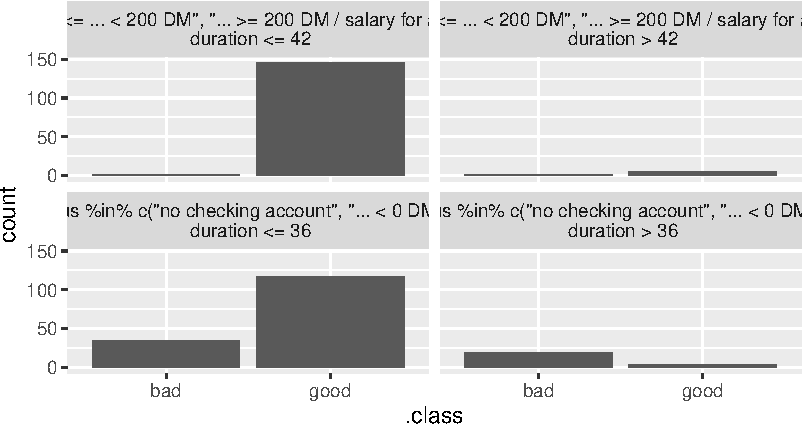
\includegraphics[width=1\textwidth,height=\textheight]{chapters/chapter12/model_interpretation_files/figure-pdf/fig-iml-surro-1.pdf}

}

\caption{\label{fig-iml-surro}Distribution of the predicted outcomes for
each terminal node identified by the tree surrogate. The top two nodes
consist of applications with a positive balance in the account
(\texttt{status}is either
\texttt{"0\ \textless{}=\ ...\ \textless{}\ 200\ DM"},
\texttt{"...\ \textgreater{}=\ 200\ DM"} or
\texttt{"salary\ for\ at\ least\ 1\ year"}) and either a duration of
less or equal than 42 months (top left), or more than 42 months (top
right). The bottom nodes contain applicants that either have no checking
account or a negative balance (\texttt{status}) and either a duration of
less than or equal to 36 months (bottom left) or more than 36 months
(bottom right).}

\end{figure}

Or we could access the trained tree surrogate via the \texttt{\$tree}
field of the \texttt{TreeSurrogate} object and then have access to all
methods in
\href{https://cran.r-project.org/package=partykit}{\texttt{partykit}}:

\begin{Shaded}
\begin{Highlighting}[]
\NormalTok{partykit}\SpecialCharTok{::}\FunctionTok{print.party}\NormalTok{(tree\_surrogate}\SpecialCharTok{$}\NormalTok{tree)}
\end{Highlighting}
\end{Shaded}

\begin{verbatim}
[1] root
|   [2] status in no checking account, ... < 0 DM
|   |   [3] duration <= 36: *
|   |   [4] duration > 36: *
|   [5] status in 0<= ... < 200 DM, ... >= 200 DM / salary for at least 1 year
|   |   [6] duration <= 42: *
|   |   [7] duration > 42: *
\end{verbatim}

\hypertarget{local-surrogate-model}{%
\subsubsection{Local Surrogate Model}\label{local-surrogate-model}}

\index{surrogate model!local}In general, it can be very difficult to
accurately approximate the black box model with an interpretable
surrogate in the entire feature space. Therefore, local surrogate models
focus on a small area in the feature space surrounding a point of
interest. Local surrogate models are constructed as follows:

\begin{enumerate}
\def\labelenumi{\arabic{enumi}.}
\tightlist
\item
  Obtain predictions from the black box model for a given dataset.
\item
  Weight the observations in this dataset by their proximity to our
  point of interest.
\item
  Fit an interpretable, surrogate model on the weighted dataset using
  the predictions of the black box model as the target.
\item
  Explain the prediction of our point of interest with the surrogate
  model.
\end{enumerate}

To illustrate this, we will select a random data point to explain. As we
are dealing with people, we will name our observation ``Charlie'' and
first look at the black box predictions:

\begin{Shaded}
\begin{Highlighting}[]
\NormalTok{Charlie }\OtherTok{=}\NormalTok{ credit\_x[}\DecValTok{35}\NormalTok{, ]}
\NormalTok{gbm\_predict }\OtherTok{=}\NormalTok{ predictor}\SpecialCharTok{$}\FunctionTok{predict}\NormalTok{(Charlie)}
\NormalTok{gbm\_predict}
\end{Highlighting}
\end{Shaded}

\begin{verbatim}
    good    bad
1 0.6346 0.3654
\end{verbatim}

We can see that the model predicts the class `good' with 63.5\%
probability, so now we can use
\href{https://www.rdocumentation.org/packages/iml/topics/LocalModel}{\texttt{LocalModel}}
to find out why this prediction was made. The underlying surrogate model
is a locally weighted L1-penalized linear regression model such that
only a pre-defined number of features per class, \texttt{k} (default is
\texttt{3}), will have a non-zero coefficient and as such are the
\texttt{k} most influential features, below we set \texttt{k\ =\ 2}. We
can also set the parameter \texttt{gower.power} which specifies the size
of the neighborhood for the local model (default is
\texttt{gower.power\ =\ 1}), the smaller the value, the more the model
will focus on points closer to the point of interest, below we set
\texttt{gower.power\ =\ 0.1}. This implementation is very closely
related to Local Interpretable Model-agnostic Explanations
(LIME\index{LIME}) (Ribeiro, Singh, and Guestrin 2016), the differences
are outlined in the documentation of \texttt{iml::LocalModel}.

\begin{Shaded}
\begin{Highlighting}[]
\NormalTok{predictor}\SpecialCharTok{$}\NormalTok{class }\OtherTok{=} \StringTok{"good"} \CommentTok{\# explain the \textquotesingle{}good\textquotesingle{} class}
\NormalTok{local\_surrogate }\OtherTok{=}\NormalTok{ LocalModel}\SpecialCharTok{$}\FunctionTok{new}\NormalTok{(predictor, Charlie, }\AttributeTok{gower.power =} \FloatTok{0.1}\NormalTok{,}
  \AttributeTok{k =} \DecValTok{2}\NormalTok{)}
\end{Highlighting}
\end{Shaded}

If the prediction of the local model and the prediction of the black box
GBM model greatly differ, then you might want to experiment with
changing the \texttt{k} and \texttt{gower.power} parameters. These
parameters can be considered as hyperparameters of the local surrogate
model, which should be tuned to obtain an accurate local surrogate.
First, we check if the predictions for Charlie match:

\begin{Shaded}
\begin{Highlighting}[]
\FunctionTok{c}\NormalTok{(}\AttributeTok{gbm =}\NormalTok{ gbm\_predict[[}\DecValTok{1}\NormalTok{]], }\AttributeTok{local =}\NormalTok{ local\_surrogate}\SpecialCharTok{$}\FunctionTok{predict}\NormalTok{()[[}\DecValTok{1}\NormalTok{]])}
\end{Highlighting}
\end{Shaded}

\begin{verbatim}
   gbm  local 
0.6346 0.6539 
\end{verbatim}

Ideally, we should assess the fidelity of the surrogate model in the
local neighborhood of Charlie, i.e., how well the local surrogate model
approximates the predictions of the black box GBM model for multiple
data points in the vicinity of Charlie. A practical approach to assess
this local model fidelity involves generating artificial data points
within Charlie's local neighborhood (and potentially applying
distance-based weighting) or selecting the \(k\) nearest neighbors from
the original data. For illustration purposes, we now quantify the
approximation error using the mean absolute error calculated from the 10
nearest neighbors (including Charlie) according to the Gower distance
(Gower 1971):

\begin{Shaded}
\begin{Highlighting}[]
\NormalTok{ind\_10nn }\OtherTok{=}\NormalTok{ gower}\SpecialCharTok{::}\FunctionTok{gower\_topn}\NormalTok{(Charlie, credit\_x, }\AttributeTok{n =} \DecValTok{10}\NormalTok{)}\SpecialCharTok{$}\NormalTok{index[, }\DecValTok{1}\NormalTok{]}
\NormalTok{Charlie\_10nn }\OtherTok{=}\NormalTok{ credit\_x[ind\_10nn, ]}

\NormalTok{gbm\_pred\_10nn }\OtherTok{=}\NormalTok{ predictor}\SpecialCharTok{$}\FunctionTok{predict}\NormalTok{(Charlie\_10nn)[[}\DecValTok{1}\NormalTok{]]}
\NormalTok{local\_pred\_10nn }\OtherTok{=}\NormalTok{ local\_surrogate}\SpecialCharTok{$}\FunctionTok{predict}\NormalTok{(Charlie\_10nn)[[}\DecValTok{1}\NormalTok{]]}
\FunctionTok{mean}\NormalTok{(}\FunctionTok{abs}\NormalTok{(gbm\_pred\_10nn }\SpecialCharTok{{-}}\NormalTok{ local\_pred\_10nn))}
\end{Highlighting}
\end{Shaded}

\begin{verbatim}
[1] 0.05475
\end{verbatim}

As we see good agreement between the local and black box model (on
average, the predictions of both the local surrogate and the black box
model for Charlie's 10 nearest neighbors differ only by 0.055), we can
move on to look at the most influential features for Charlie's
predictions:

\begin{Shaded}
\begin{Highlighting}[]
\NormalTok{local\_surrogate}\SpecialCharTok{$}\NormalTok{results[, }\FunctionTok{c}\NormalTok{(}\StringTok{"feature.value"}\NormalTok{, }\StringTok{"effect"}\NormalTok{)]}
\end{Highlighting}
\end{Shaded}

\begin{verbatim}
               feature.value   effect
1                duration=12 -0.02000
2 status=no checking account -0.08544
\end{verbatim}

In this case, `duration' and `status' were most important and both have
a negative effect on the prediction of Charlie.

\hypertarget{sec-shapley}{%
\subsection{Shapley Values}\label{sec-shapley}}

Shapley values\index{Shapley values} were originally developed in the
context of cooperative game theory to study how the payout of a game can
be fairly distributed among the players that form a team. This concept
has been adapted for use in ML as a local interpretation method to
explain the contributions of each input feature to the final model
prediction of a single observation (Štrumbelj and Kononenko 2013).
Hence, the `players' are the features, and the `payout', which should be
fairly distributed among features, refers to the difference between the
individual observation's prediction and the mean prediction.

Shapley values estimate how much each input feature contributed to the
final prediction for a single observation (after subtracting the mean
prediction). By assigning a value to each feature, we can gain insights
into which features were the most important ones for the considered
observation. Compared to the penalized linear model as a local surrogate
model, Shapley values guarantee that the prediction is fairly
distributed among the features as they also inherently consider
interactions between features when calculating the contribution of each
feature.

\begin{tcolorbox}[enhanced jigsaw, opacitybacktitle=0.6, rightrule=.15mm, opacityback=0, arc=.35mm, breakable, titlerule=0mm, colframe=quarto-callout-warning-color-frame, coltitle=black, bottomrule=.15mm, toprule=.15mm, colback=white, colbacktitle=quarto-callout-warning-color!10!white, bottomtitle=1mm, toptitle=1mm, title=\textcolor{quarto-callout-warning-color}{\faExclamationTriangle}\hspace{0.5em}{Correctly Interpreting Shapley Values}, leftrule=.75mm, left=2mm]

Shapley values are frequently \textbf{misinterpreted} as the difference
between the predicted value after removing the feature from model
training. The Shapley value of a feature is calculated by considering
all possible subsets of features and computing the difference in the
model prediction with and without the feature of interest included.
Hence, it refers to the average marginal contribution of a feature to
the difference between the actual prediction and the mean prediction,
given the current set of features.

\end{tcolorbox}

Shapley values can be calculated by passing the \texttt{Predictor} and
the observation of interest to the constructor of
\href{https://www.rdocumentation.org/packages/iml/topics/Shapley}{\texttt{Shapley}}.
The exact computation of Shapley values is time consuming, as it
involves taking into account all possible combinations of features to
calculate the marginal contribution of a feature. Therefore, the
estimation of Shapley values is often approximated. The
\texttt{sample.size} argument (default is \texttt{sample.size\ =\ 100})
can be increased to obtain a more accurate approximation of exact
Shapley values.

\begin{Shaded}
\begin{Highlighting}[]
\NormalTok{shapley }\OtherTok{=}\NormalTok{ Shapley}\SpecialCharTok{$}\FunctionTok{new}\NormalTok{(predictor, }\AttributeTok{x.interest =}\NormalTok{ Charlie,}
  \AttributeTok{sample.size =} \DecValTok{1000}\NormalTok{)}
\NormalTok{shapley}\SpecialCharTok{$}\FunctionTok{plot}\NormalTok{()}
\end{Highlighting}
\end{Shaded}

\begin{figure}[H]

{\centering 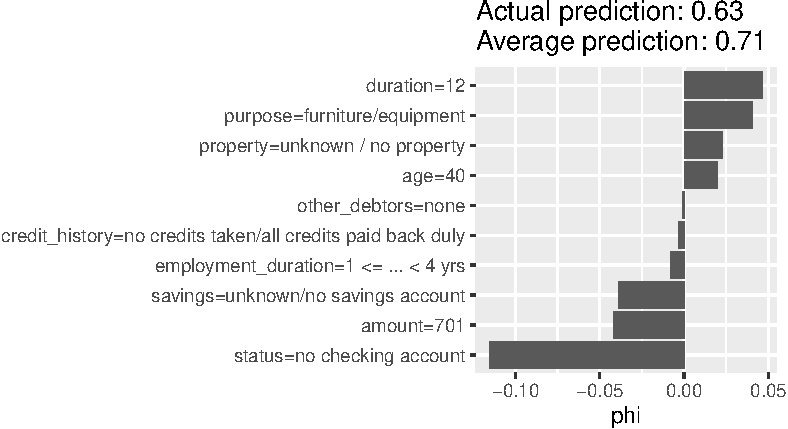
\includegraphics[width=1\textwidth,height=\textheight]{chapters/chapter12/model_interpretation_files/figure-pdf/fig-iml-shapley-1.pdf}

}

\caption{\label{fig-iml-shapley}Shapley values for Charlie. The actual
prediction (0.63) displays the prediction of the model for the
observation we are interested in, the average prediction (0.71) displays
the average prediction over the given test dataset. Each horizontal bar
is the Shapley value (phi) for the given feature.}

\end{figure}

In Figure~\ref{fig-iml-shapley}, the Shapley values (\texttt{phi}) of
the features show us how to fairly distribute the difference of
Charlie's probability of being creditworthy to the dataset's average
probability among the given features. The approximation is sufficiently
good if all Shapley values (\texttt{phi}) sum up to the difference of
the actual prediction and the average prediction. Here, we used
\texttt{sample.size\ =\ 1000} leading to sufficiently good prediction
difference of -0.079 between the actual prediction of Charlie (0.635)
and the average prediction (0.706). The `purpose' variable has the most
positive effect on the probability of being creditworthy, with an
increase in the predicted probability of around 5\%. In contrast, the
`status' variable leads to a decrease in the predicted probability of
over 10\%.

\hypertarget{sec-counterfactuals}{%
\section{The counterfactuals Package}\label{sec-counterfactuals}}

\index{\texttt{counterfactuals}}Counterfactual\index{counterfactual}
explanations try to identify the smallest possible changes to the input
features of a given observation that would lead to a different
prediction (Wachter, Mittelstadt, and Russell 2017). In other words, a
counterfactual explanation provides an answer to the question: ``What
changes in the current feature values are necessary to achieve a
different prediction?''.

Counterfactual explanations can have many applications in different
areas such as healthcare, finance, and criminal justice, where it may be
important to understand how small changes in input features could affect
the model's prediction. For example, a counterfactual explanation could
be used to suggest lifestyle changes to a patient to reduce their risk
of developing a particular disease, or to suggest actions that would
increase the chance of a credit being approved. For our
\texttt{tsk("german\_credit")} example, we might consider what changes
in features would turn a `bad' credit prediction into a `good' one
(Figure~\ref{fig-counterfactuals-ill}).

\begin{figure}

{\centering 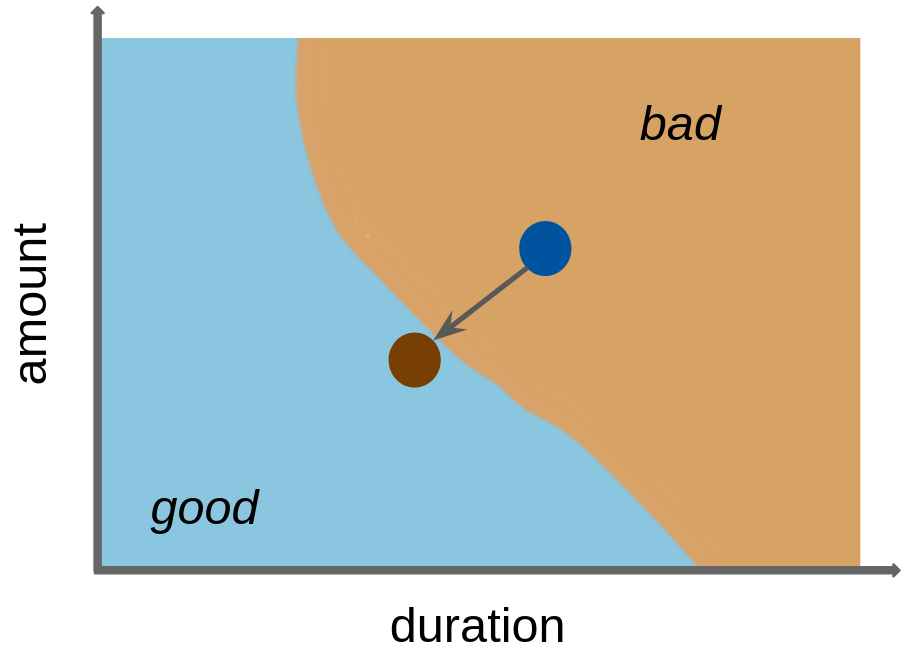
\includegraphics[width=0.5\textwidth,height=\textheight]{chapters/chapter12/Figures/counterfactuals.png}

}

\caption{\label{fig-counterfactuals-ill}Illustration of a counterfactual
explanation. The real observation (blue, right dot) is predicted to have
`bad' credit. The brown (left) dot is one possible counterfactual that
would result in a `good' credit prediction.}

\end{figure}

A simple counterfactual method is the
What-If\index{What-If}{\marginnote{\begin{footnotesize}What-If\end{footnotesize}}}
approach (Wexler et al. 2019) where, for a given prediction to explain,
the counterfactual is the closest data point in the dataset with the
desired prediction. Usually, many possible counterfactual data points
can exist. However, the approach by Wexler et al. (2019), and several
other early counterfactual methods (see Guidotti (2022) for a
comprehensive overview), only produce a single, somewhat arbitrary
counterfactual explanation, which can be regarded as problematic when
counterfactuals are used for insights or actions against the model.

In contrast, the multi-objective
counterfactuals\index{multi-objective counterfactuals}{\marginnote{\begin{footnotesize}Multi-objective
Counterfactuals\end{footnotesize}}} method (MOC) (Dandl et al. 2020)
generates multiple artificially-generated counterfactuals that may not
be equal to observations in a given dataset. The generation of
counterfactuals is based on an optimization problem that aims for
counterfactuals that:

\begin{enumerate}
\def\labelenumi{\arabic{enumi})}
\tightlist
\item
  Have the desired prediction;
\item
  Are close to the observation of interest;
\item
  Only require changes in a few features; and
\item
  Originate from the same distribution as the observations in the given
  dataset.
\end{enumerate}

In MOC, all four objectives are optimized simultaneously via a
multi-objective optimization method. Several other counterfactual
methods rely on single-objective optimization methods, where multiple
objectives are combined into a single objective, e.g., using a weighted
sum. However, a single-objective approach raises concerns about the
appropriate weighting of objectives and is unable to account for
inherent trade-offs among individual objectives. Moreover, it may
restrict the solution set of the counterfactural search to a single
candidate. MOC returns a set of non-dominated and, therefore equally
good, counterfactuals with respect to the four objectives (similarly to
the Pareto front\index{Pareto front} we saw in
Section~\ref{sec-multi-metrics-tuning}).

Counterfactual explanations are available in the
\texttt{counterfactuals} package, which depends on
\href{https://www.rdocumentation.org/packages/iml/topics/Predictor}{\texttt{Predictor}}
objects as inputs.

\hypertarget{what-if-method}{%
\subsection{What-If Method}\label{what-if-method}}

Continuing our previous example, we saw that the GBM model classifies
Charlie as having good credit with a predicted probability of 63.5\%. We
can use the What-If method to understand how the features need to change
for this predicted probability to increase to 75\%. We initialize a
\href{https://www.rdocumentation.org/packages/counterfactuals/topics/WhatIfClassif}{\texttt{WhatIfClassif}}
object with our \texttt{Predictor} and state that we only want to find
one counterfactual (\texttt{n\_counterfactuals\ =\ 1L}), increasing
\texttt{n\_counterfactuals} would return the specified number of
counterfactuals closest to the point of interest. The
\texttt{\$find\_counterfactuals()} method generates a counterfactual of
class
\href{https://www.rdocumentation.org/packages/counterfactuals/topics/Counterfactuals}{\texttt{Counterfactuals}},
below we set our desired predicted probability to be between
\texttt{0.75} and \texttt{1} (\texttt{desired\_prob\ =\ c(0.75,\ 1)}).
The \texttt{\$evaluate(show\_diff\ =\ TRUE)} method tells us how
features need to be changed to generate our desired class.

\begin{Shaded}
\begin{Highlighting}[]
\FunctionTok{library}\NormalTok{(counterfactuals)}
\NormalTok{whatif }\OtherTok{=}\NormalTok{ WhatIfClassif}\SpecialCharTok{$}\FunctionTok{new}\NormalTok{(predictor, }\AttributeTok{n\_counterfactuals =}\NormalTok{ 1L)}
\NormalTok{cfe }\OtherTok{=}\NormalTok{ whatif}\SpecialCharTok{$}\FunctionTok{find\_counterfactuals}\NormalTok{(Charlie,}
  \AttributeTok{desired\_class =} \StringTok{"good"}\NormalTok{, }\AttributeTok{desired\_prob =} \FunctionTok{c}\NormalTok{(}\FloatTok{0.75}\NormalTok{, }\DecValTok{1}\NormalTok{))}
\FunctionTok{data.frame}\NormalTok{(cfe}\SpecialCharTok{$}\FunctionTok{evaluate}\NormalTok{(}\AttributeTok{show\_diff =} \ConstantTok{TRUE}\NormalTok{))}
\end{Highlighting}
\end{Shaded}

\begin{verbatim}
  age amount credit_history duration employment_duration other_debtors
1  -3   1417           <NA>       -3                <NA>          <NA>
  property purpose savings     status dist_x_interest no_changed
1     <NA>    <NA>    <NA> ... < 0 DM          0.1176          4
  dist_train dist_target minimality
1          0           0          1
\end{verbatim}

Here we can see that, to achieve a predicted probability of at least
75\% for good credit, Charlie would have to be three years younger, the
duration of credit would have to be reduced by three months, the amount
would have to be increased by 1417 DM and the status would have to be
`\ldots{} \textless{} 0 DM' (instead of `no checking account') .

\hypertarget{moc-method}{%
\subsection{MOC Method}\label{moc-method}}

Calling the MOC method is similar to the What-If method but with a
\href{https://www.rdocumentation.org/packages/counterfactuals/topics/MOCClassif}{\texttt{MOCClassif()}}
object. We set the \texttt{epsilon} parameter to 0 to penalize
counterfactuals in the optimization process with predictions outside the
desired range. With MOC, we can also prohibit changes in specific
features via the \texttt{fixed\_features} argument, below we restrict
changes in the `age' variable. For illustrative purposes, we only run
the multi-objective optimizer for 30 generations.

\begin{Shaded}
\begin{Highlighting}[]
\NormalTok{moc }\OtherTok{=}\NormalTok{ MOCClassif}\SpecialCharTok{$}\FunctionTok{new}\NormalTok{(predictor, }\AttributeTok{epsilon =} \DecValTok{0}\NormalTok{, }\AttributeTok{n\_generations =}\NormalTok{ 30L,}
  \AttributeTok{fixed\_features =} \StringTok{"age"}\NormalTok{)}
\NormalTok{cfe\_multi }\OtherTok{=}\NormalTok{ moc}\SpecialCharTok{$}\FunctionTok{find\_counterfactuals}\NormalTok{(Charlie,}
  \AttributeTok{desired\_class =} \StringTok{"good"}\NormalTok{, }\AttributeTok{desired\_prob =} \FunctionTok{c}\NormalTok{(}\FloatTok{0.75}\NormalTok{, }\DecValTok{1}\NormalTok{))}
\end{Highlighting}
\end{Shaded}

The multi-objective approach does not guarantee that all counterfactuals
have the desired prediction so we use \texttt{\$subset\_to\_valid()} to
restrict counterfactuals to those we are interested in:

\begin{Shaded}
\begin{Highlighting}[]
\NormalTok{cfe\_multi}\SpecialCharTok{$}\FunctionTok{subset\_to\_valid}\NormalTok{()}
\NormalTok{cfe\_multi}
\end{Highlighting}
\end{Shaded}

\begin{verbatim}
6 Counterfactual(s) 
 
Desired class: good 
Desired predicted probability range: [0.75, 1] 
 
Head: 
   age amount                              credit_history duration
1:  40    701 no credits taken/all credits paid back duly       12
2:  40    701 no credits taken/all credits paid back duly       12
3:  40    701 no credits taken/all credits paid back duly       12
6 variables not shown: [employment_duration, other_debtors, property, purpose, savings, status]
\end{verbatim}

This method generated 6 counterfactuals but as these are artificially
generated they are not necessarily equal to actual observations in the
underlying dataset. For a concise overview of the required feature
changes, we can use the \texttt{plot\_freq\_of\_feature\_changes()}
method, which visualizes the frequency of feature changes across all
returned counterfactuals.

\begin{Shaded}
\begin{Highlighting}[]
\NormalTok{cfe\_multi}\SpecialCharTok{$}\FunctionTok{plot\_freq\_of\_feature\_changes}\NormalTok{()}
\end{Highlighting}
\end{Shaded}

\begin{figure}[H]

{\centering 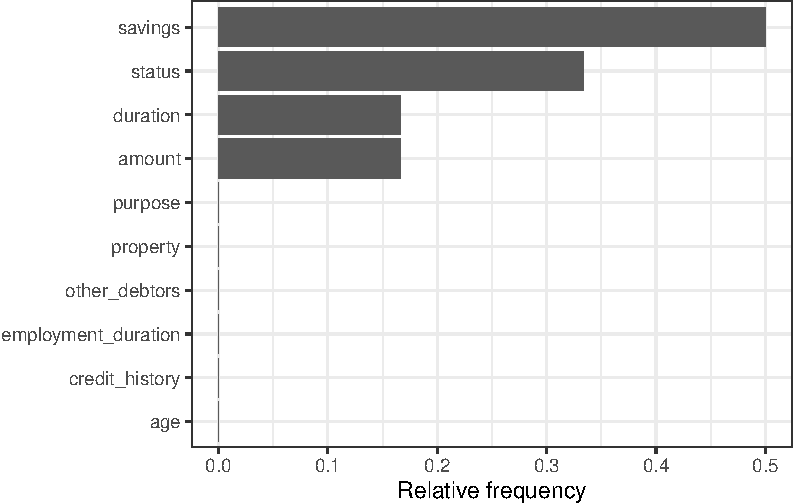
\includegraphics[width=1\textwidth,height=\textheight]{chapters/chapter12/model_interpretation_files/figure-pdf/fig-cf-mocfreq-1.pdf}

}

\caption{\label{fig-cf-mocfreq}Barplots of the relative frequency of
feature changes of the counterfactuals found by MOC.}

\end{figure}

We can see that `status' and `savings' were changed most frequently in
the counterfactuals. To see \emph{how} the features were changed, we can
visualize the counterfactuals for two features on a two-dimensional ICE
plot.

\begin{Shaded}
\begin{Highlighting}[]
\NormalTok{cfe\_multi}\SpecialCharTok{$}\FunctionTok{plot\_surface}\NormalTok{(}\AttributeTok{feature\_names =} \FunctionTok{c}\NormalTok{(}\StringTok{"status"}\NormalTok{, }\StringTok{"savings"}\NormalTok{)) }\SpecialCharTok{+}
    \FunctionTok{theme}\NormalTok{(}\AttributeTok{axis.text.x =} \FunctionTok{element\_text}\NormalTok{(}\AttributeTok{angle =} \DecValTok{15}\NormalTok{, }\AttributeTok{hjust =}\NormalTok{ .}\DecValTok{7}\NormalTok{))}
\end{Highlighting}
\end{Shaded}

\begin{figure}[H]

{\centering 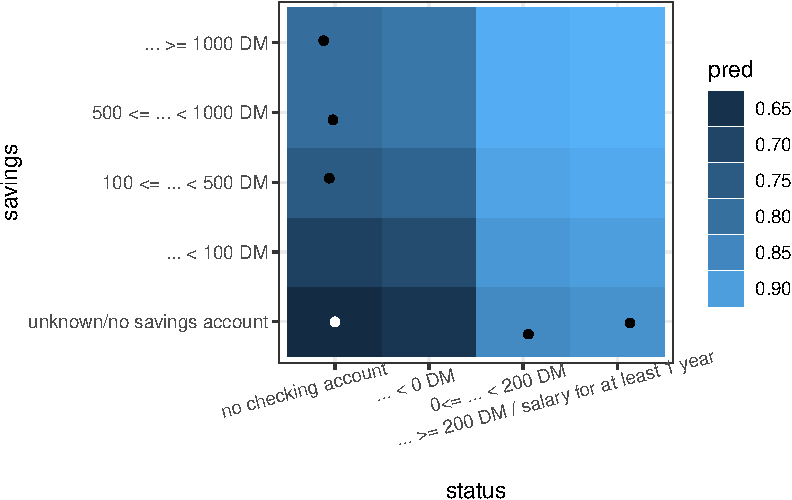
\includegraphics[width=1\textwidth,height=\textheight]{chapters/chapter12/model_interpretation_files/figure-pdf/fig-cf-mocsurface-1.pdf}

}

\caption{\label{fig-cf-mocsurface}Two-dimensional surface plot for the
`status' and `savings' variables, higher predictions are lighter. The
colors and contour lines indicate the predicted value of the model when
`status' and `savings' differ while all other features are set to the
true (Charlie's) values. The white point displays the true prediction
(Charlie), and the black points are the counterfactuals that only
propose changes in the two features.}

\end{figure}

\hypertarget{sec-dalex}{%
\section{\texorpdfstring{The \texttt{DALEX}
Package}{The DALEX Package}}\label{sec-dalex}}

\href{https://cran.r-project.org/package=DALEX}{\texttt{DALEX}}\index{\texttt{DALEX}}
(Biecek 2018) implements a similar set of methods as \texttt{iml}, but
the architecture of \texttt{DALEX} is oriented towards model comparison.
The logic behind working with this package assumes that the process of
exploring models is iterative, and in successive iterations, we want to
compare different perspectives, including perspectives presented/learned
by different models. This logic is commonly referred to as the
Rashomon\index{Rashomon} perspective, first described in Breiman (2001b)
and more extensively developed and formalized as interactive explanatory
model analysis (Baniecki, Parzych, and Biecek 2023).

You can use the \texttt{DALEX} package with any classification and
regression model built with \texttt{mlr3} as well as with other
frameworks in R. As we have already explored the methodology behind most
of the methods discussed in this section, we will just focus on the
implementations of these methods in \texttt{DALEX} using the
\texttt{tsk("german\_credit")} running example.

Once you become familiar with the philosophy of working with the
\texttt{DALEX} package, you can use other packages from this family such
as
\href{https://cran.r-project.org/package=fairmodels}{\texttt{fairmodels}}
(Wiśniewski and Biecek 2022) for detection and mitigation of biases,
\href{https://cran.r-project.org/package=modelStudio}{\texttt{modelStudio}}
(Baniecki and Biecek 2019) for interactive model exploration,
\href{https://cran.r-project.org/package=modelDown}{\texttt{modelDown}}
(Romaszko et al. 2019) for the automatic generation of IML model
documentation,
\href{https://cran.r-project.org/package=survex}{\texttt{survex}}
(Krzyziński et al. 2023) for the explanation of survival models, or
\href{https://cran.r-project.org/package=treeshap}{\texttt{treeshap}}
for the analysis of tree-based models.

The analysis of a model is usually an interactive process starting with
evaluating a model based on one or more performance metrics, known as a
`shallow analysis'. In a series of subsequent steps, one can
systematically deepen understanding of the model by exploring the
importance of single variables or pairs of variables to an in-depth
analysis of the relationship between selected variables to the model
outcome. See Bücker et al. (2022) for a broader discussion of what the
model exploration process looks like.

This explanatory model
analysis\index{explanatory model analysis}{\marginnote{\begin{footnotesize}Explanatory
Model Analysis\end{footnotesize}}} (EMA) process can focus on a single
observation, in which case we speak of local model analysis, or for a
set of observations, in which case we refer to global model analysis.
Figure~\ref{fig-dalex-fig-plot-01} visualizes an overview of the key
functions in these two scenarios that we will discuss in this section.
An in-depth description of this methodology can be found in Biecek and
Burzykowski (2021).

\begin{figure}

{\centering 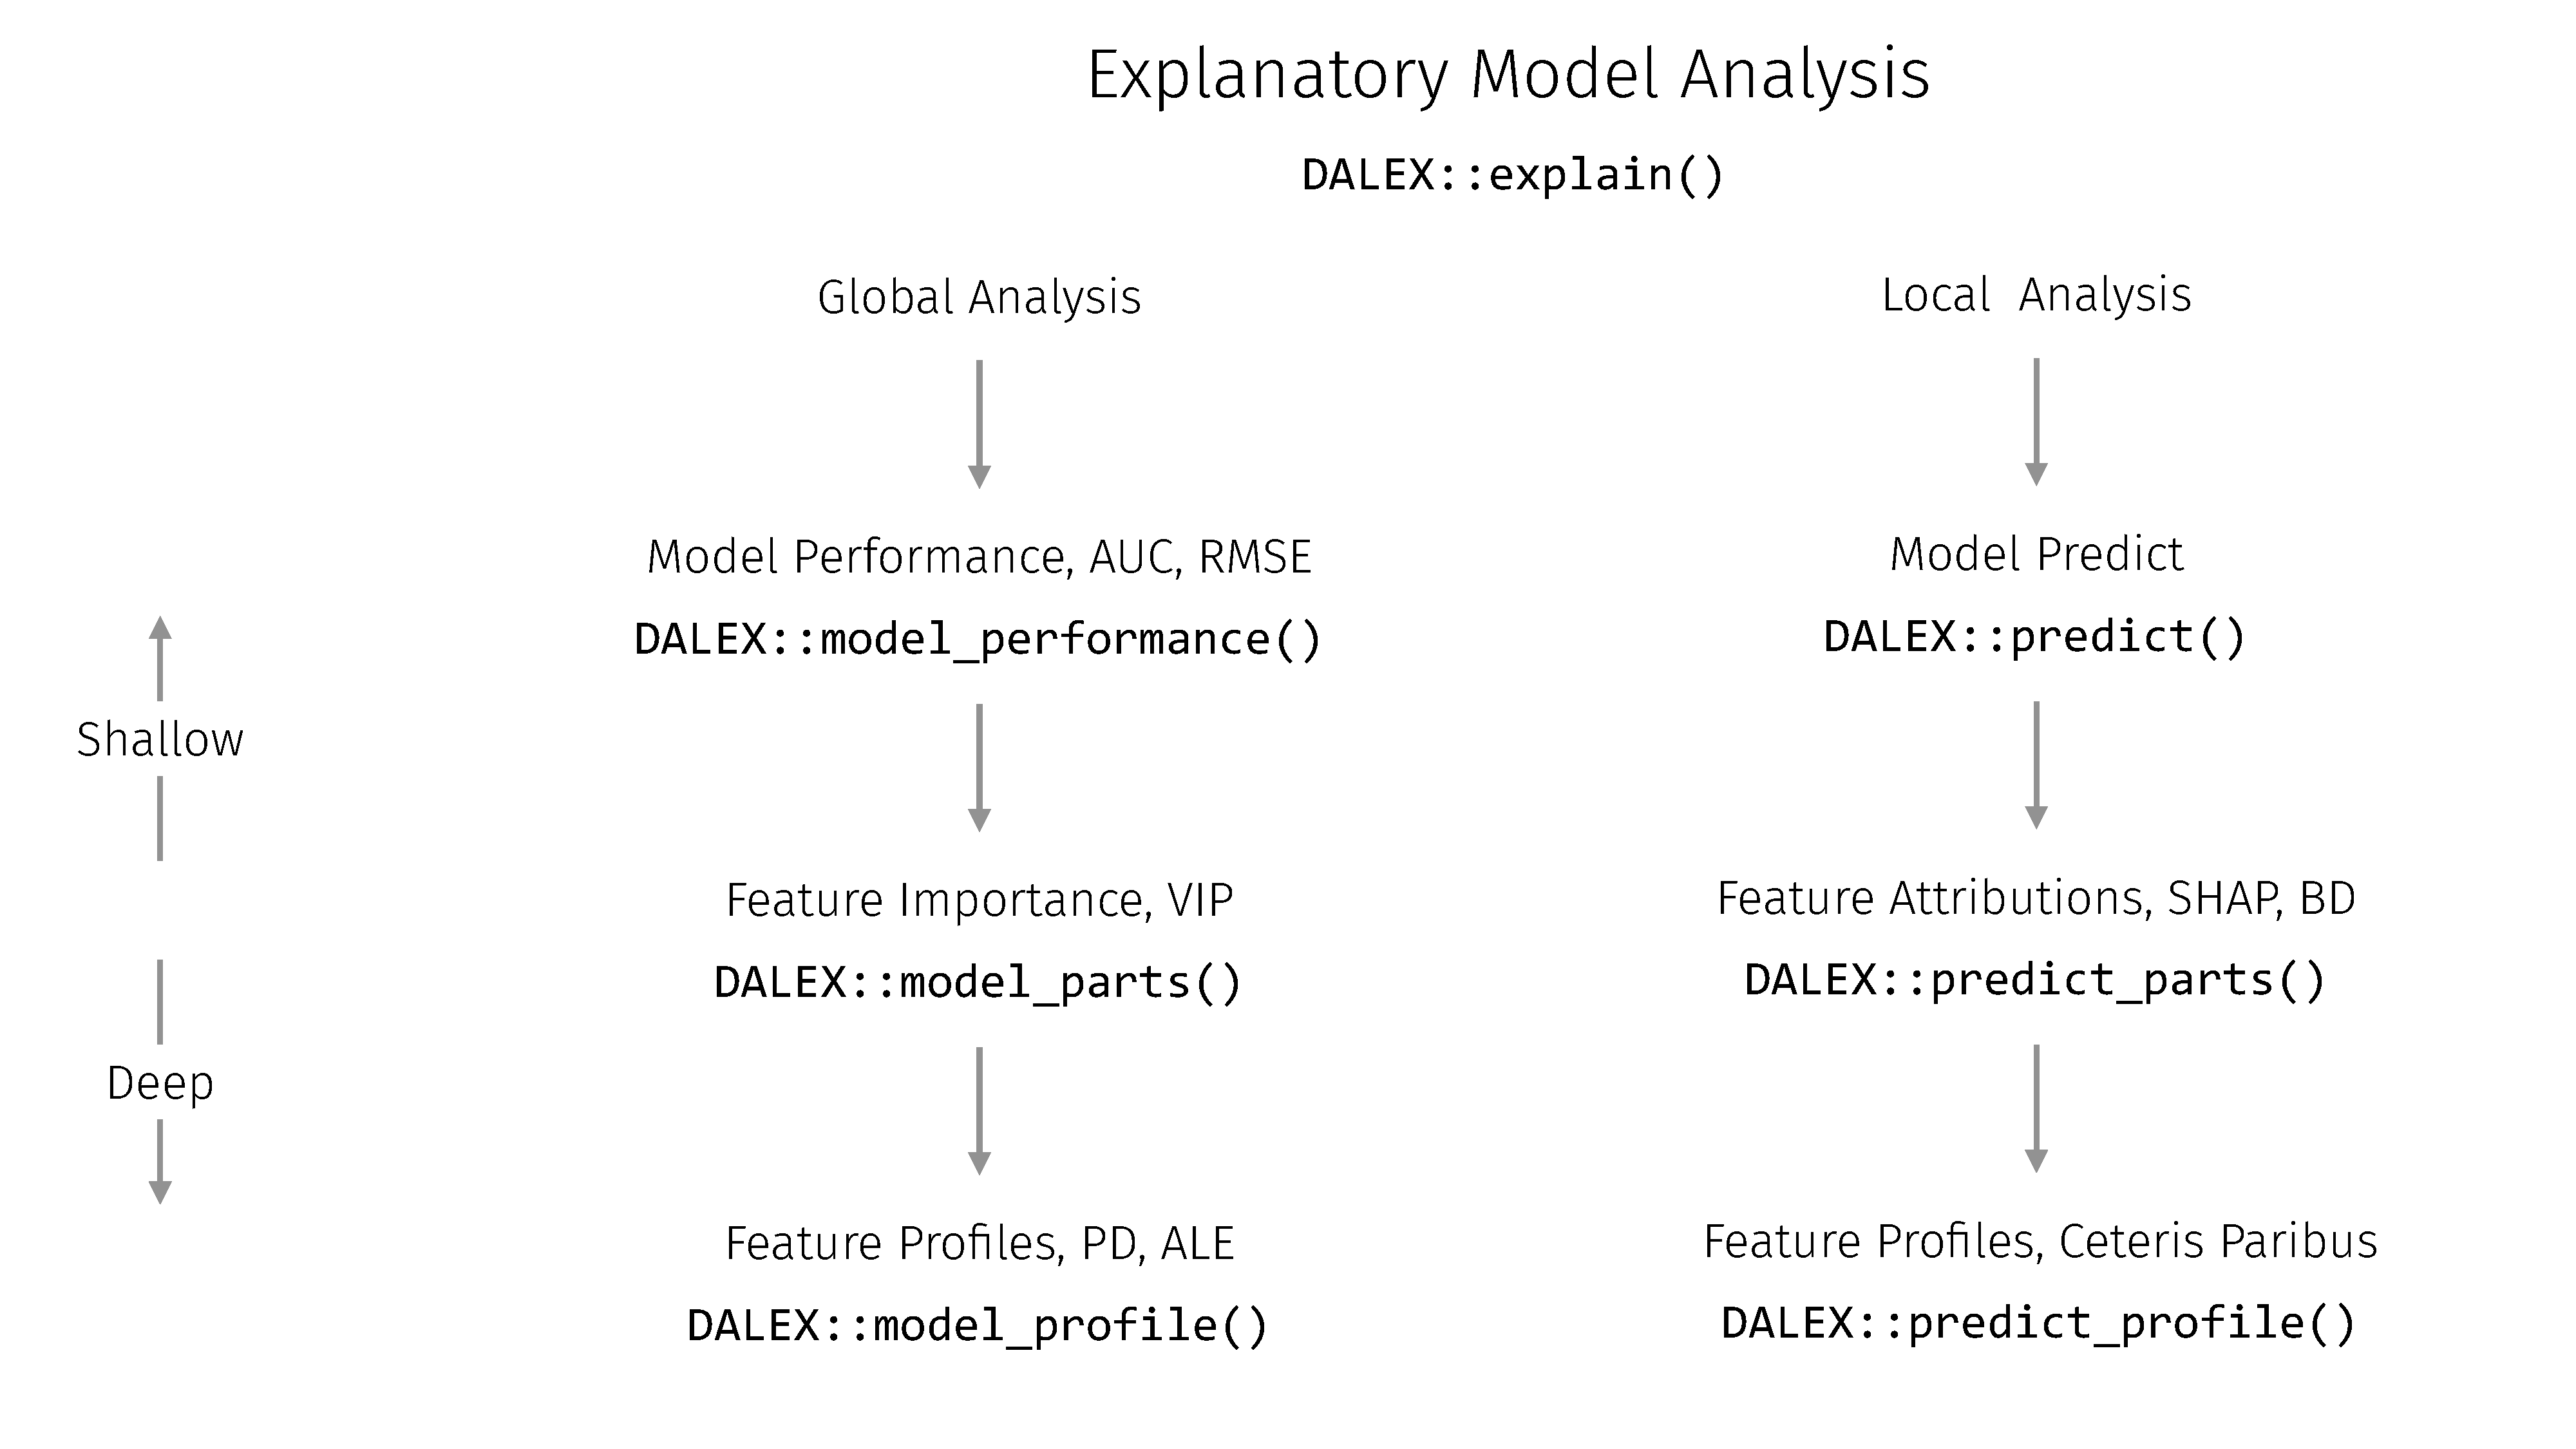
\includegraphics[width=0.92\textwidth,height=\textheight]{chapters/chapter12/Figures/DALEX_ema_process.pdf}

}

\caption{\label{fig-dalex-fig-plot-01}Taxonomy of methods for model
exploration presented in this section. The left side shows global
analysis methods and the right shows local analysis methods. Methods
increase in analysis complexity from top to bottom.}

\end{figure}

As with \texttt{iml}, \texttt{DALEX} also implements a wrapper that
enables a unified interface to its functionality. For models created
with the \texttt{mlr3} package, we would use
\href{https://www.rdocumentation.org/packages/DALEXtra/topics/explain_mlr3}{\texttt{explain\_mlr3()}},
which creates an S3 \texttt{explainer} object, which is a list
containing at least: the model object, the dataset that will be used for
calculation of explanations, the predict function, the function that
calculates residuals, name/label of the model name and other additional
information about the model.

\begin{Shaded}
\begin{Highlighting}[]
\FunctionTok{library}\NormalTok{(DALEX)}
\FunctionTok{library}\NormalTok{(DALEXtra)}

\NormalTok{gbm\_exp }\OtherTok{=}\NormalTok{ DALEXtra}\SpecialCharTok{::}\FunctionTok{explain\_mlr3}\NormalTok{(lrn\_gbm,}
  \AttributeTok{data =}\NormalTok{ credit\_x,}
  \AttributeTok{y =} \FunctionTok{as.numeric}\NormalTok{(credit\_y}\SpecialCharTok{$}\NormalTok{credit\_risk }\SpecialCharTok{==} \StringTok{"bad"}\NormalTok{),}
  \AttributeTok{label =} \StringTok{"GBM Credit"}\NormalTok{,}
  \AttributeTok{colorize =} \ConstantTok{FALSE}\NormalTok{)}

\NormalTok{gbm\_exp}
\end{Highlighting}
\end{Shaded}

\begin{verbatim}
Model label:  GBM Credit 
Model class:  LearnerClassifGBM,LearnerClassif,Learner,R6 
Data head  :
  age amount                          credit_history duration
1  67   1169 all credits at this bank paid back duly        6
2  49   2096 all credits at this bank paid back duly       12
  employment_duration other_debtors              property
1            >= 7 yrs          none unknown / no property
2    4 <= ... < 7 yrs          none unknown / no property
              purpose                    savings
1 furniture/equipment             ... >= 1000 DM
2             repairs unknown/no savings account
                                      status
1                        no checking account
2 ... >= 200 DM / salary for at least 1 year
\end{verbatim}

\hypertarget{sec-interpretability-dataset-level}{%
\subsection{Global EMA}\label{sec-interpretability-dataset-level}}

Global EMA aims to understand how a model behaves on average for a set
of observations. In \texttt{DALEX}, functions for global level analysis
are prefixed with \texttt{model\_}.

The model exploration process starts
(Figure~\ref{fig-dalex-fig-plot-01}) by evaluating the performance of a
model.
\href{https://www.rdocumentation.org/packages/DALEX/topics/model_performance}{\texttt{model\_performance()}}
detects the task type and selects the most appropriate measure, as we
are using binary classification the function automatically suggests
recall, precision, F1-score, accuracy, and AUC; similarly the default
plotting method is selected based on the task type, below ROC is
selected.

\begin{Shaded}
\begin{Highlighting}[]
\NormalTok{perf\_credit }\OtherTok{=} \FunctionTok{model\_performance}\NormalTok{(gbm\_exp)}
\NormalTok{perf\_credit}
\end{Highlighting}
\end{Shaded}

\begin{verbatim}
Measures for:  classification
recall     : 0.3535 
precision  : 0.614 
f1         : 0.4487 
accuracy   : 0.7394 
auc        : 0.7689

Residuals:
      0%      10%      20%      30%      40%      50%      60%      70% 
-0.88117 -0.44188 -0.31691 -0.20743 -0.14601 -0.10782 -0.07089  0.03232 
     80%      90%     100% 
 0.49779  0.65661  0.94458 
\end{verbatim}

\begin{Shaded}
\begin{Highlighting}[]
\NormalTok{old\_theme }\OtherTok{=} \FunctionTok{set\_theme\_dalex}\NormalTok{(}\StringTok{"ema"}\NormalTok{)}
\FunctionTok{plot}\NormalTok{(perf\_credit, }\AttributeTok{geom =} \StringTok{"roc"}\NormalTok{)}
\end{Highlighting}
\end{Shaded}

\begin{figure}

{\centering 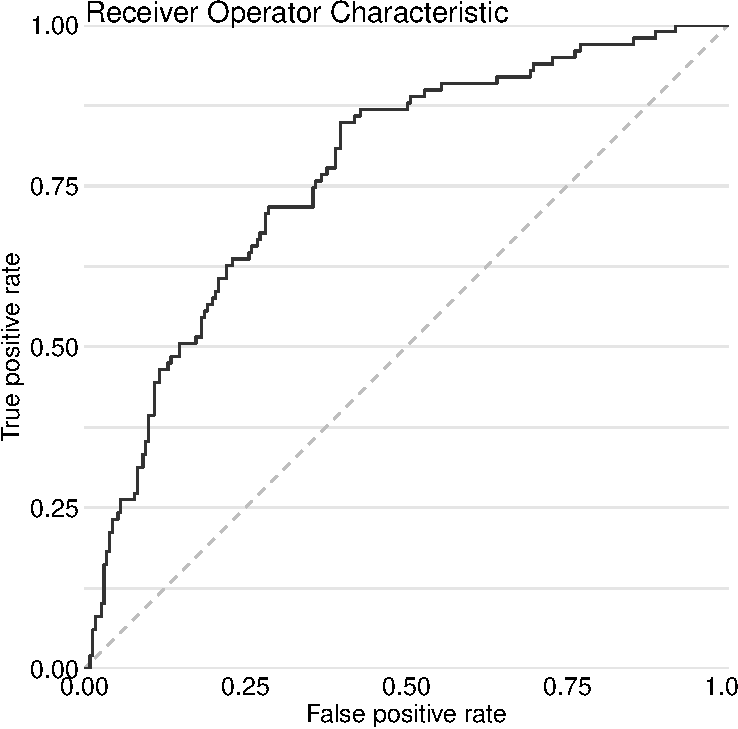
\includegraphics[width=0.6\textwidth,height=\textheight]{chapters/chapter12/model_interpretation_files/figure-pdf/fig-dalex-roc-1.pdf}

}

\caption{\label{fig-dalex-roc}Graphical summary of model performance
using the Receiver Operator Curve (Section~\ref{sec-roc}).}

\end{figure}

\begin{tcolorbox}[enhanced jigsaw, opacitybacktitle=0.6, rightrule=.15mm, opacityback=0, arc=.35mm, breakable, titlerule=0mm, colframe=quarto-callout-tip-color-frame, coltitle=black, bottomrule=.15mm, toprule=.15mm, colback=white, colbacktitle=quarto-callout-tip-color!10!white, bottomtitle=1mm, toptitle=1mm, title=\textcolor{quarto-callout-tip-color}{\faLightbulb}\hspace{0.5em}{Visual Summaries}, leftrule=.75mm, left=2mm]

Various visual summaries may be selected with the \texttt{geom}
parameter. For the credit risk task, the LIFT curve is a popular
graphical summary.

\end{tcolorbox}

Feature importance methods can be calculated with
\href{https://www.rdocumentation.org/packages/DALEX/topics/model_parts}{\texttt{model\_parts()}}
and then plotted.

\begin{Shaded}
\begin{Highlighting}[]
\NormalTok{gbm\_effect }\OtherTok{=} \FunctionTok{model\_parts}\NormalTok{(gbm\_exp)}
\FunctionTok{head}\NormalTok{(gbm\_effect)}
\end{Highlighting}
\end{Shaded}

\begin{verbatim}
             variable mean_dropout_loss      label
1        _full_model_            0.2311 GBM Credit
2       other_debtors            0.2351 GBM Credit
3              amount            0.2351 GBM Credit
4            property            0.2353 GBM Credit
5                 age            0.2355 GBM Credit
6 employment_duration            0.2403 GBM Credit
\end{verbatim}

\begin{Shaded}
\begin{Highlighting}[]
\FunctionTok{plot}\NormalTok{(gbm\_effect, }\AttributeTok{show\_boxplots =} \ConstantTok{FALSE}\NormalTok{)}
\end{Highlighting}
\end{Shaded}

\begin{figure}

{\centering 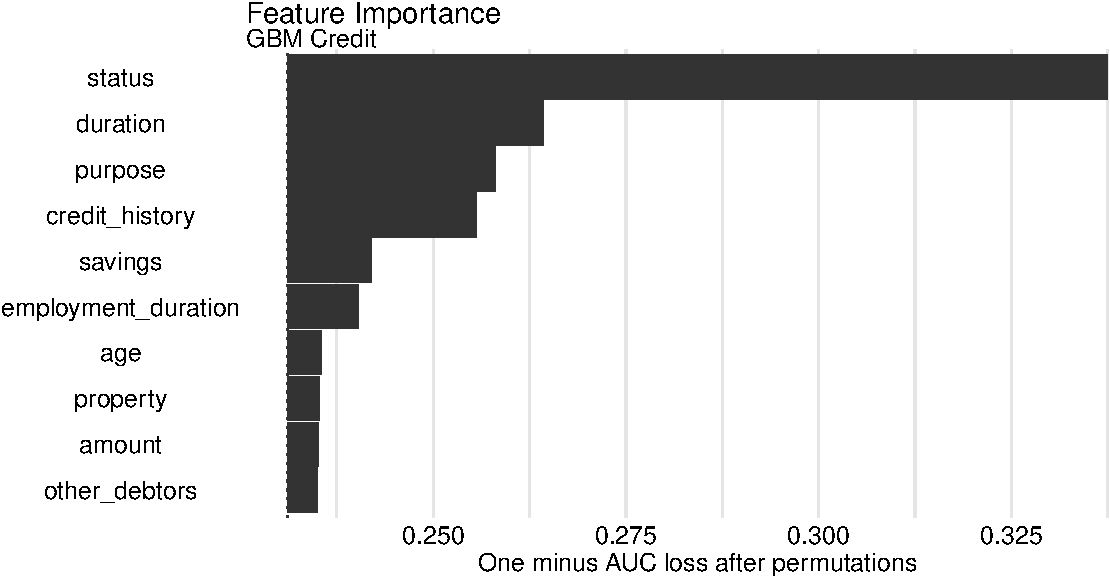
\includegraphics[width=0.9\textwidth,height=\textheight]{chapters/chapter12/model_interpretation_files/figure-pdf/fig-dalex-featimp-1.pdf}

}

\caption{\label{fig-dalex-featimp}Graphical summary of permutation
importance of features. The longer the bar, the larger the change in the
loss function after permutation of the particular feature and therefore
the more important the feature. This plot shows that `status' is the
most important feature and `other\_debtors' is the least important.}

\end{figure}

\begin{tcolorbox}[enhanced jigsaw, opacitybacktitle=0.6, rightrule=.15mm, opacityback=0, arc=.35mm, breakable, titlerule=0mm, colframe=quarto-callout-tip-color-frame, coltitle=black, bottomrule=.15mm, toprule=.15mm, colback=white, colbacktitle=quarto-callout-tip-color!10!white, bottomtitle=1mm, toptitle=1mm, title=\textcolor{quarto-callout-tip-color}{\faLightbulb}\hspace{0.5em}{Calculating Importance}, leftrule=.75mm, left=2mm]

The \texttt{type} argument in the \texttt{model\_parts} function allows
you to specify how the importance of the features is to be calculated,
by the difference of the loss functions
(\texttt{type\ =\ "difference"}), by the quotient
(\texttt{type\ =\ "ratio"}), or without any transformation
(\texttt{type\ =\ "raw"}).

\end{tcolorbox}

Feature effects can be calculated with
\href{https://www.rdocumentation.org/packages/DALEX/topics/model_profile}{\texttt{model\_profile()}}
and by default are plotted as PD plots.

\begin{Shaded}
\begin{Highlighting}[]
\NormalTok{gbm\_profiles }\OtherTok{=} \FunctionTok{model\_profile}\NormalTok{(gbm\_exp)}
\NormalTok{gbm\_profiles}
\end{Highlighting}
\end{Shaded}

\begin{verbatim}
Top profiles    : 
   _vname_    _label_ _x_ _yhat_ _ids_
1 duration GBM Credit   4 0.2052     0
2 duration GBM Credit   6 0.2052     0
3 duration GBM Credit   7 0.2052     0
4 duration GBM Credit   8 0.2052     0
5 duration GBM Credit   9 0.2246     0
6 duration GBM Credit  10 0.2246     0
\end{verbatim}

\begin{Shaded}
\begin{Highlighting}[]
\FunctionTok{plot}\NormalTok{(gbm\_profiles) }\SpecialCharTok{+}
  \FunctionTok{theme}\NormalTok{(}\AttributeTok{legend.position =} \StringTok{"top"}\NormalTok{) }\SpecialCharTok{+}
  \FunctionTok{ggtitle}\NormalTok{(}\StringTok{"Partial Dependence for GBM Credit model"}\NormalTok{,}\StringTok{""}\NormalTok{)}
\end{Highlighting}
\end{Shaded}

\begin{figure}

{\centering 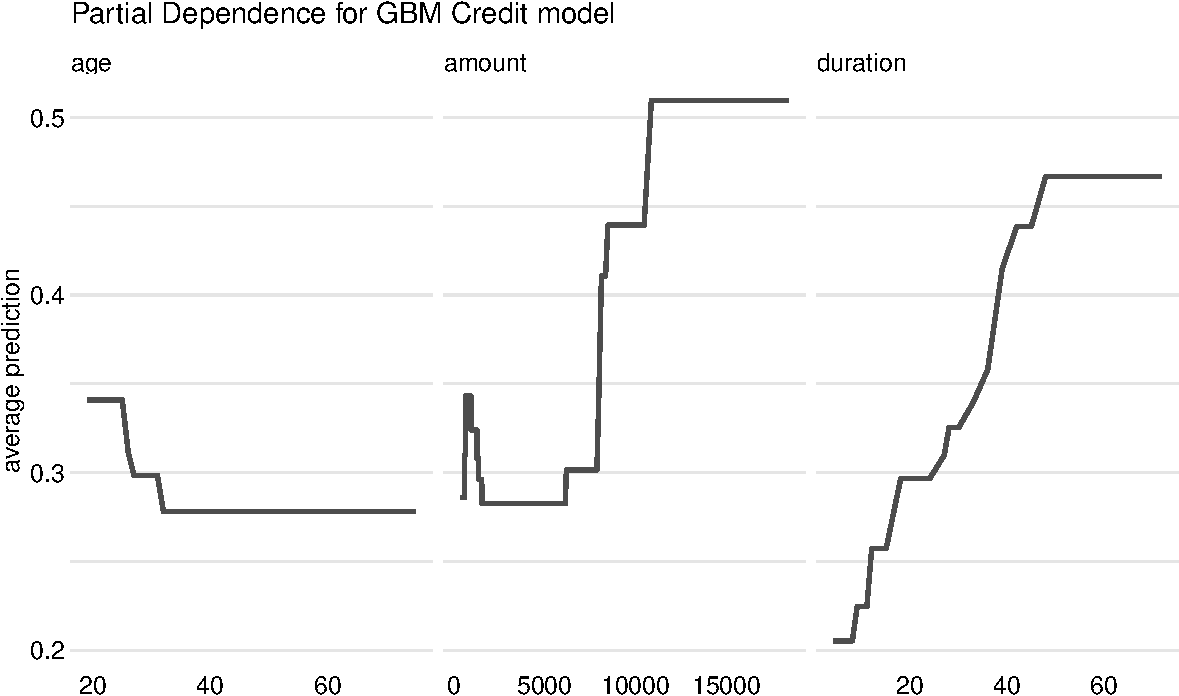
\includegraphics[width=0.9\textwidth,height=\textheight]{chapters/chapter12/model_interpretation_files/figure-pdf/fig-dalex-pdp-1.pdf}

}

\caption{\label{fig-dalex-pdp}Graphical summary of the model's partial
dependence profile for three selected variables (age, amount,
duration).}

\end{figure}

From Figure~\ref{fig-dalex-pdp}, we can see that the GBM model has
learned a non-monotonic relationship for the feature \texttt{amount}.

\begin{tcolorbox}[enhanced jigsaw, opacitybacktitle=0.6, rightrule=.15mm, opacityback=0, arc=.35mm, breakable, titlerule=0mm, colframe=quarto-callout-tip-color-frame, coltitle=black, bottomrule=.15mm, toprule=.15mm, colback=white, colbacktitle=quarto-callout-tip-color!10!white, bottomtitle=1mm, toptitle=1mm, title=\textcolor{quarto-callout-tip-color}{\faLightbulb}\hspace{0.5em}{Marginal and Accumulated Local Profiles}, leftrule=.75mm, left=2mm]

The \texttt{type} argument of the
\href{https://www.rdocumentation.org/packages/DALEX/topics/model_profile}{\texttt{model\_profile()}}
function also allows \emph{marginal profiles} (with
\texttt{type\ =\ "conditional"}) and \emph{accumulated local profiles}
(with \texttt{type\ =\ "accumulated"}) to be calculated.

\end{tcolorbox}

\hypertarget{sec-interpretability-instance-level}{%
\subsection{Local EMA}\label{sec-interpretability-instance-level}}

Local EMA aims to understand how a model behaves for a single
observation. In \texttt{DALEX}, functions for local analysis are
prefixed with \texttt{predict\_}. We will carry out the following
examples using Charlie again.

Local analysis starts with the calculation of a model prediction
(Figure~\ref{fig-dalex-fig-plot-01}).

\begin{Shaded}
\begin{Highlighting}[]
\FunctionTok{predict}\NormalTok{(gbm\_exp, Charlie)}
\end{Highlighting}
\end{Shaded}

\begin{verbatim}
   bad 
0.3654 
\end{verbatim}

As a next step, we might consider break-down plots, which decompose the
model's prediction into contributions that can be attributed to
different explanatory variables (see the \emph{Break-down Plots for
Additive Attributions} chapter in Biecek and Burzykowski (2021) for more
on this method). These are calculated with
\href{https://www.rdocumentation.org/packages/DALEX/topics/predict_parts}{\texttt{predict\_parts()}}:

\begin{Shaded}
\begin{Highlighting}[]
\FunctionTok{plot}\NormalTok{(}\FunctionTok{predict\_parts}\NormalTok{(gbm\_exp, }\AttributeTok{new\_observation =}\NormalTok{ Charlie))}
\end{Highlighting}
\end{Shaded}

\begin{figure}[H]

{\centering 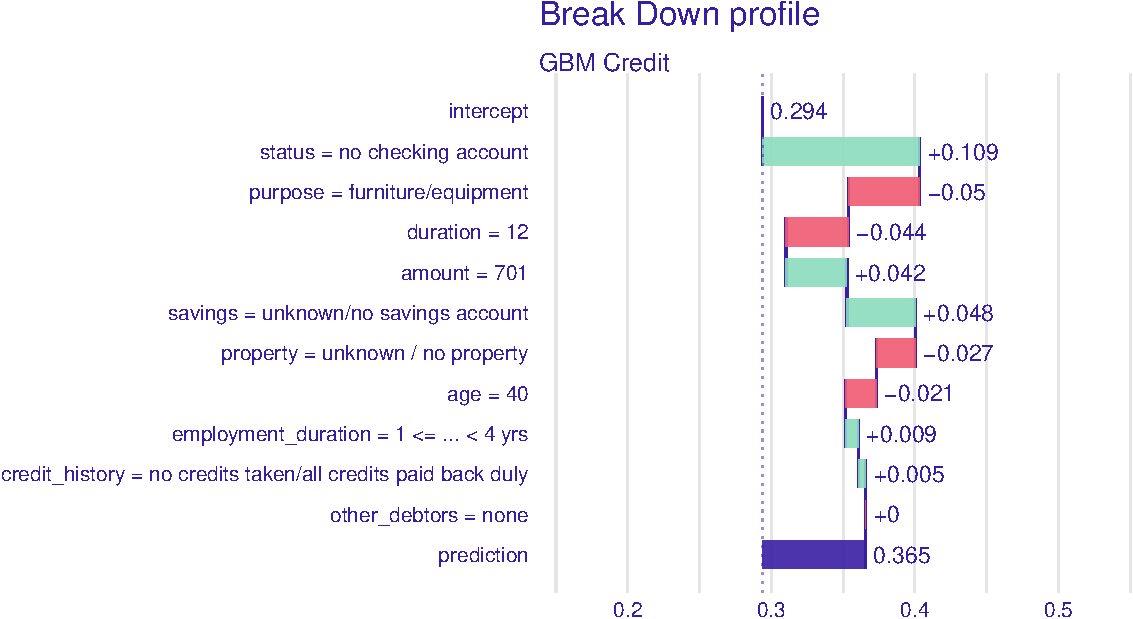
\includegraphics[width=0.9\textwidth,height=\textheight]{chapters/chapter12/model_interpretation_files/figure-pdf/fig-dalex-breakdown-1.pdf}

}

\caption{\label{fig-dalex-breakdown}Graphical summary of local
attributions of features calculated by the break-down method. Positive
attributions are shown in green and negative attributions in red. The
violet bar corresponds to the model prediction for the explained
observation and the dashed line corresponds to the average model
prediction.}

\end{figure}

Looking at Figure~\ref{fig-dalex-breakdown}, we can read that the
biggest contributors to the final prediction for Charlie were the
features \texttt{status} and \texttt{savings}.

\begin{tcolorbox}[enhanced jigsaw, opacitybacktitle=0.6, rightrule=.15mm, opacityback=0, arc=.35mm, breakable, titlerule=0mm, colframe=quarto-callout-tip-color-frame, coltitle=black, bottomrule=.15mm, toprule=.15mm, colback=white, colbacktitle=quarto-callout-tip-color!10!white, bottomtitle=1mm, toptitle=1mm, title=\textcolor{quarto-callout-tip-color}{\faLightbulb}\hspace{0.5em}{Selected Order of Features}, leftrule=.75mm, left=2mm]

The \texttt{order} argument allows you to indicate the selected order of
the features. This is a useful option when the features have some
relative conditional importance (e.g.~pregnancy and sex).

\end{tcolorbox}

The \texttt{predict\_parts()} function can also be used to plot Shapley
values with the SHAP algorithm (Lundberg, Erion, and Lee 2019) by
setting \texttt{type\ =\ "shap"}:

\begin{Shaded}
\begin{Highlighting}[]
\FunctionTok{plot}\NormalTok{(}\FunctionTok{predict\_parts}\NormalTok{(gbm\_exp, }\AttributeTok{new\_observation =}\NormalTok{ Charlie, }\AttributeTok{type =} \StringTok{"shap"}\NormalTok{),}
  \AttributeTok{show\_boxplots =} \ConstantTok{FALSE}\NormalTok{)}
\end{Highlighting}
\end{Shaded}

\begin{figure}[H]

{\centering 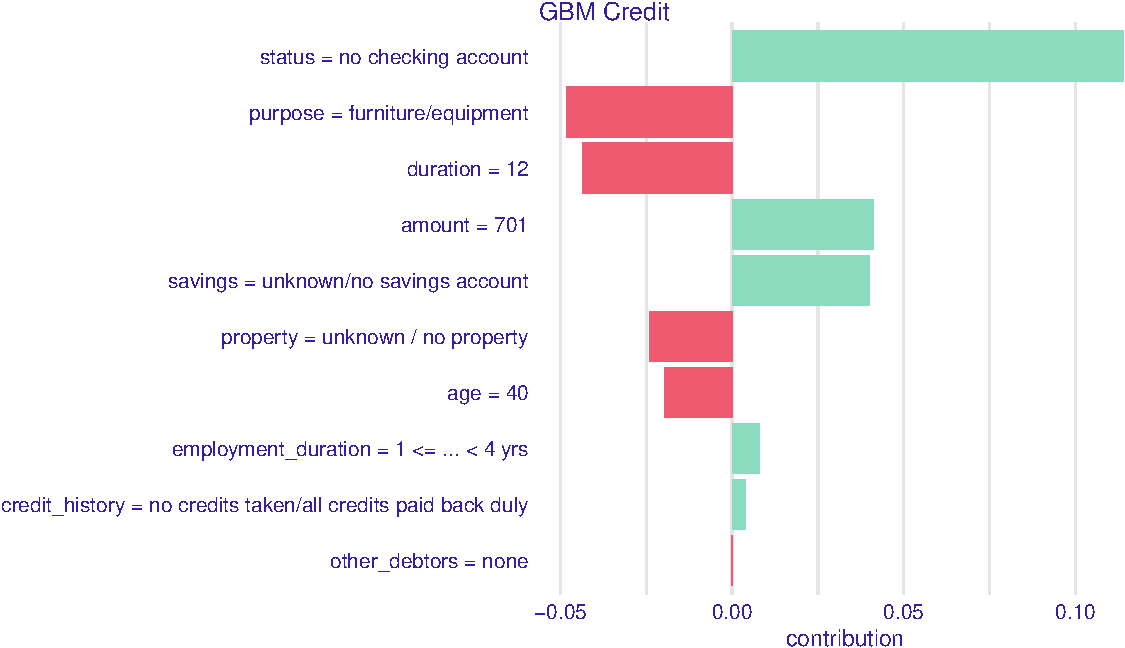
\includegraphics[width=0.9\textwidth,height=\textheight]{chapters/chapter12/model_interpretation_files/figure-pdf/fig-dalex-shaps-1.pdf}

}

\caption{\label{fig-dalex-shaps}Graphical summary of local attributions
of features calculated by the Shap method. Positive attributions are
shown in green and negative attributions in red. The most important
feature here is the `status' variable and least is `other\_debtors'.}

\end{figure}

The results for Break Down and SHAP methods are generally similar.
Differences will emerge if there are many complex interactions in the
model.

\begin{tcolorbox}[enhanced jigsaw, opacitybacktitle=0.6, rightrule=.15mm, opacityback=0, arc=.35mm, breakable, titlerule=0mm, colframe=quarto-callout-tip-color-frame, coltitle=black, bottomrule=.15mm, toprule=.15mm, colback=white, colbacktitle=quarto-callout-tip-color!10!white, bottomtitle=1mm, toptitle=1mm, title=\textcolor{quarto-callout-tip-color}{\faLightbulb}\hspace{0.5em}{Speeding Up Shapley Computation}, leftrule=.75mm, left=2mm]

Shapley values can take a long time to compute. This process can be sped
up at the expense of accuracy. The parameters \texttt{B} and \texttt{N}
can be used to tune this trade-off, where \texttt{N} is the number of
observations on which conditional expectation values are estimated (500
by default) and \texttt{B} is the number of random paths used to
calculate Shapley values (25 by default).

\end{tcolorbox}

Finally, we can plot ICE curves using
\href{https://www.rdocumentation.org/packages/DALEX/topics/predict_profile}{\texttt{predict\_profile()}}:

\begin{Shaded}
\begin{Highlighting}[]
\FunctionTok{plot}\NormalTok{(}\FunctionTok{predict\_profile}\NormalTok{(gbm\_exp,  credit\_x[}\DecValTok{30}\SpecialCharTok{:}\DecValTok{40}\NormalTok{, ]))}
\end{Highlighting}
\end{Shaded}

\begin{figure}[H]

{\centering 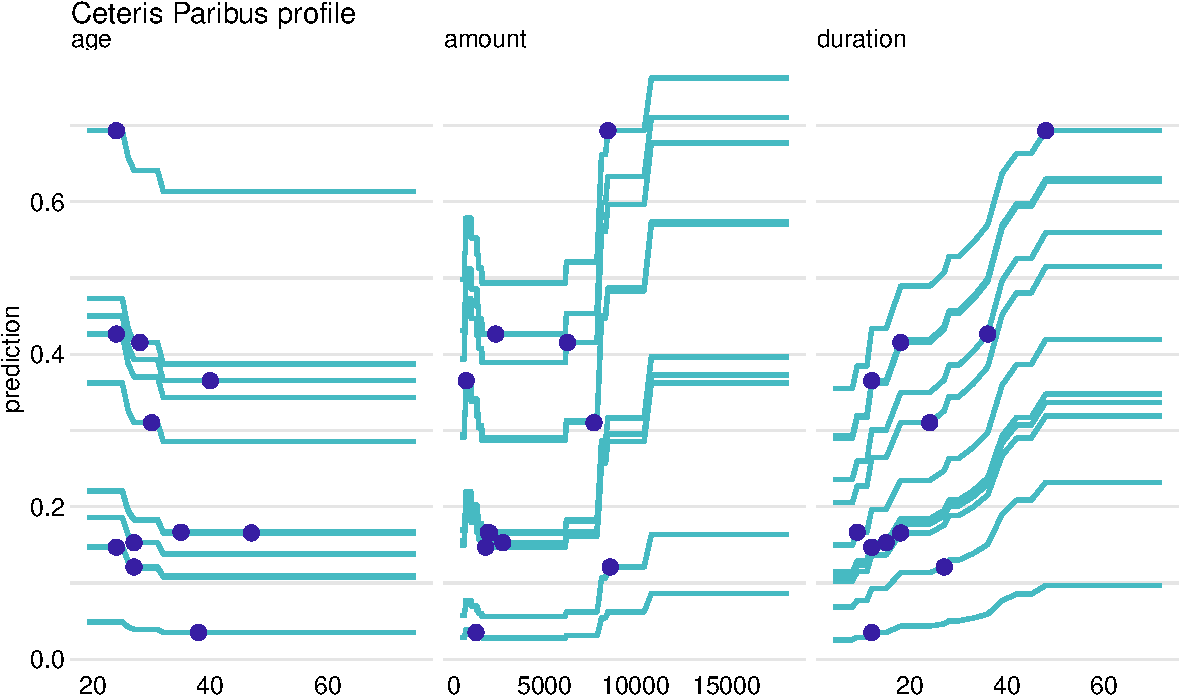
\includegraphics[width=0.9\textwidth,height=\textheight]{chapters/chapter12/model_interpretation_files/figure-pdf/fig-dalex-ice-1.pdf}

}

\caption{\label{fig-dalex-ice}Individual conditional explanations (aka
Ceteris Paribus) plots for 10 rows in the credit data (including
Charlie) for three selected variables (age, amount, duration).}

\end{figure}

\hypertarget{conclusions}{%
\section{Conclusions}\label{conclusions}}

In this chapter, we learned how to gain post hoc insights into a model
trained with \texttt{mlr3} by using the most popular approaches from the
field of interpretable machine learning. The methods are all
model-agnostic and so do not depend on specific model classes.
\href{https://cran.r-project.org/package=iml}{\texttt{iml}} and
\href{https://cran.r-project.org/package=DALEX}{\texttt{DALEX}} offer a
wide range of (partly) overlapping methods, while
\href{https://cran.r-project.org/package=counterfactuals}{\texttt{counterfactuals}}
focuses solely on counterfactual methods. We demonstrated on
\texttt{tsk("german\_credit")} how these packages offer an in-depth
analysis of a GBM model fitted with \texttt{mlr3}. As we conclude the
chapter we will highlight some limitations in the methods discussed
above to help guide your own post hoc analyses.

\hypertarget{correlated-features}{%
\subsubsection*{Correlated Features}\label{correlated-features}}

If features are correlated, the insights from the interpretation methods
should be treated with caution. Changing the feature values of an
observation without taking the correlation with other features into
account leads to unrealistic combinations of the feature values. Since
such feature combinations are also unlikely to be part of the training
data, the model will likely extrapolate in these areas (Molnar et al.
2022; Hooker and Mentch 2019). This distorts the interpretation of
methods that are based on changing single feature values such as PFI, PD
plots, and Shapley values. Alternative methods can help in these cases:
conditional feature importance instead of PFI (Strobl et al. 2008;
Watson and Wright 2021), accumulated local effect plots instead of PD
plots (Apley and Zhu 2020), and the KernelSHAP method instead of Shapley
values (Lundberg, Erion, and Lee 2019).

\hypertarget{rashomon-effect}{%
\subsubsection*{Rashomon Effect}\label{rashomon-effect}}

Explanations derived from an interpretation method can be ambiguous. A
method can deliver multiple equally plausible but potentially
contradicting explanations. This phenomenon is also called the
Rashomon\index{Rashomon} effect (Breiman 2001b). This effect can be due
to changes in hyperparameters, the underlying dataset, or even the
initial seed (Molnar et al. 2022).

\hypertarget{high-dimensional-data}{%
\subsubsection*{High-Dimensional Data}\label{high-dimensional-data}}

\texttt{tsk("german\_credit")} is low-dimensional with a limited number
of observations. Applying interpretation methods off-the-shelf to higher
dimensional datasets is often not feasible due to the enormous
computational costs and so recent methods, such as Shapley values that
use kernel-based estimators, have been developed to help over come this.
Another challenge is that the high-dimensional IML output generated for
high-dimensional datasets can overwhelm users. If the features can be
meaningfully grouped, grouped versions of methods, e.g.~the grouped
feature importance proposed by Au et al. (2022), can be applied.

\hypertarget{tbl-interpretation-api}{}
\begin{longtable}[]{@{}
  >{\raggedright\arraybackslash}p{(\columnwidth - 4\tabcolsep) * \real{0.4286}}
  >{\raggedright\arraybackslash}p{(\columnwidth - 4\tabcolsep) * \real{0.2857}}
  >{\raggedright\arraybackslash}p{(\columnwidth - 4\tabcolsep) * \real{0.2857}}@{}}
\caption{\label{tbl-interpretation-api}Important classes and functions
covered in this chapter with underlying class (if applicable), class
constructor or function, and important class fields and methods (if
applicable).}\tabularnewline
\toprule\noalign{}
\begin{minipage}[b]{\linewidth}\raggedright
Class
\end{minipage} & \begin{minipage}[b]{\linewidth}\raggedright
Constructor/Function
\end{minipage} & \begin{minipage}[b]{\linewidth}\raggedright
Fields/Methods
\end{minipage} \\
\midrule\noalign{}
\endfirsthead
\toprule\noalign{}
\begin{minipage}[b]{\linewidth}\raggedright
Class
\end{minipage} & \begin{minipage}[b]{\linewidth}\raggedright
Constructor/Function
\end{minipage} & \begin{minipage}[b]{\linewidth}\raggedright
Fields/Methods
\end{minipage} \\
\midrule\noalign{}
\endhead
\bottomrule\noalign{}
\endlastfoot
\href{https://www.rdocumentation.org/packages/iml/topics/Predictor}{\texttt{Predictor}}
& \texttt{\$new()} & - \\
\href{https://www.rdocumentation.org/packages/iml/topics/FeatureImp}{\texttt{FeatureImp}}
& \texttt{\$new(some\_predictor)} & \texttt{\$plot()} \\
\href{https://www.rdocumentation.org/packages/iml/topics/FeatureEffect}{\texttt{FeatureEffect}}
& \texttt{\$new(some\_predictor)} & \texttt{\$plot()} \\
\href{https://www.rdocumentation.org/packages/iml/topics/LocalModel}{\texttt{LocalModel}}
& \texttt{\$new(some\_predictor,\ some\_x)} & \texttt{\$results()} \\
\href{https://www.rdocumentation.org/packages/iml/topics/Shapley}{\texttt{Shapley}}
& \texttt{\$new(some\_predictor,\ x.interest)} & \texttt{\$plot()} \\
\href{https://www.rdocumentation.org/packages/counterfactuals/topics/WhatIfClassif}{\texttt{WhatIfClassif}}
& \texttt{\$new(some\_predictor)} &
\texttt{\$find\_counterfactuals()} \\
\href{https://www.rdocumentation.org/packages/counterfactuals/topics/MOCClassif}{\texttt{MOCClassif}}
& \texttt{\$new(some\_predictor)} &
\texttt{\$find\_counterfactuals()} \\
\href{https://www.rdocumentation.org/packages/DALEX/topics/explainer}{\texttt{explainer}}
&
\href{https://www.rdocumentation.org/packages/DALEXtra/topics/explain_mlr3}{\texttt{explain\_mlr3()}}
& \texttt{model\_parts()}; \texttt{model\_performance()};
\texttt{predict\_parts()} \\
\end{longtable}

\hypertarget{exercises-10}{%
\section{Exercises}\label{exercises-10}}

The following exercises are based on predictions of the value of soccer
players based on their characteristics in the FIFA video game series.
They use the 2020 \texttt{fifa} data available in DALEX.
Solve them with either \texttt{iml} or \texttt{DALEX}.

\begin{enumerate}
\def\labelenumi{\arabic{enumi}.}
\tightlist
\item
  Prepare an \texttt{mlr3} regression task for the \texttt{fifa} data.
  Select only features describing the age and skills of soccer players.
  Train a predictive model of your own choice on this task, to predict
  the value of a soccer player.
\item
  Use the permutation importance method to calculate feature importance
  ranking. Which feature is the most important? Do you find the results
  surprising?
\item
  Use the partial dependence plot/profile to draw the global behavior of
  the model for this feature. Is it aligned with your expectations?
\item
  Choose Manuel Neuer as a specific example and calculate and plot the
  Shapley values. Which feature is locally the most important and has
  the strongest influence on his valuation as a soccer player? Calculate
  the ceteris paribus profiles / individual conditional expectation
  curves to visualize the local behavior of the model for this feature.
  Is it different from the global behavior?
\end{enumerate}
